% !Mode:: "Tex:UTF-8"


Continuando con nuestro recorrido por la Tabla \ref{tabla:MetodosInferencia2Variables} (ver pág. \pageref{tabla:MetodosInferencia2Variables}), en la que describíamos cuatro posibles casos  de la relación entre dos variables, le llega el turno al caso C $\sim$ C, cuando tanto la variable respuesta como la explicativa son cualitativas (factores). La técnica nueva que vamos a aprender en este capítulo se conoce habitualmente como test o contraste de hipótesis $\chi^2$ (léase {\em ji cuadrado o chi cuadrado}). Vamos a ver dos aplicaciones de esta técnica. La primera de ellas, el estudio de la relación entre dos factores que ya hemos anunciado. En la segunda, tendremos una muestra,  que supuestamente procede de una distribución de probabilidad conocida, y trataremos de averiguar si los datos de la muestra se corresponden o no con esa presunta distribución teórica. Para que el lector pueda ir pensando en un ejemplo concreto, queremos desarrollar un método que nos permita averiguar si un dado está {\em cargado}.  Para ello lanzaríamos el dado muchas veces, y trataríamos de ver si las frecuencias relativas de los seis resultados posibles se parecen {\em satisfactoriamente} al valor teórico, que es $1/6$.  ¿Qué tiene que pasar para que pensemos que esa distribución de las frecuencias relativas es {\em significativamente} distinta de la esperada? El contraste $\chi^2$ nos dará la respuesta a esta pregunta, y a otras tan interesantes como la verificación experimental de las predicciones de las leyes de Mendel para la Genética.


\section{Relación entre dos factores. Tablas de contingencia y contraste $\chi^2$ de independencia.}
\label{cap12:sec:TablasContingencia}

Empecemos con el estudio de los modelos $C \sim C$ para la relación entre dos factores. Para describir esas relaciones se utilizan, como ya hemos visto,  las {\sf tablas de contingencia}\index{tablas de contingencia}. Nos hemos encontrado con ellas varias veces a lo largo del curso, desde el Ejemplo \ref{cap03:ejem:PruebasDiagnosticas01} (pág. \pageref{cap03:ejem:PruebasDiagnosticas01}), en el que las presentamos para ilustrar la noción de probabilidad condicionada, y hablábamos de pruebas diagnósticas para una enfermedad. También utilizamos ese ejemplo de las pruebas diagnósticas en la Sección \ref{cap09:sec:RiesgoRelativoCocienteProbabilidades} (pág. \pageref{cap09:sec:RiesgoRelativoCocienteProbabilidades}), y lo analizamos mediante el riesgo relativo y el cociente de probabilidades, usando el lenguaje de las tablas de contingencia. Nos vamos a encontrar de nuevo, en este capítulo, con las pruebas diagnósticas, porque esa situación es un ejemplo muy sencillo y que usa un lenguaje fácil de entender para todos nosotros, del tipo de modelo $C \sim C$ que vamos a analizar a continuación. En el caso de las pruebas diagnósticas tenemos dos factores:
\begin{itemize}
  \item $E$, el factor {\em enfermedad} con dos niveles, que son {\em enfermo} y {\em sano}.
  \item $P$, el factor {\em prueba}, que describe el resultado de la prueba, y que puede ser {\em positivo} o {\em negativo}.
\end{itemize}
Naturalmente, esperamos que haya alguna relación entre ambos factores, de manera que el resultado de la prueba en un paciente nos permita {\em predecir} cuál de los dos valores de $E$ (enfermo o sano) corresponde a ese paciente. Como se ve, la situación tiene los ingredientes comunes al tipo de problemas que estamos investigando en esta parte del curso. Es, además, un ejemplo especialmente sencillo, porque los dos factores ($E$ y $P$) tienen cada uno de ellos dos niveles (enfermo/sano, positivo/negativo). Es decir, que la tabla de contingencia es una tabla $2\times2$. En el próximo apartado vamos a comenzar con otro ejemplo de tabla de contingencia $2\times2$, distinto del de las pruebas diagnósticas, que usaremos para introducir las ideas básicas de este capítulo.

\subsection{Tablas de contingencia $2\times 2$.}
\label{cap12:subsec:TablasContingencia2x2}

\noindent Este es el ejemplo:
\begin{ejemplo}
\label{cap12:ejem:BarometroCIS01}
El\, {\em Barómetro} del CIS (Centro de Investigaciones
Sociológicas, ver el enlace [\,\ref{enlace0026}\,]\label{enlace0026a}) permite,
entre otras muchas cosas, obtener datos sobre las creencias religiosas de la población en España.
Una pregunta que puede interesarnos es ¿hay alguna diferencia al respecto entre hombres y mujeres?
Vamos a utilizar los datos del {\em Barómetro} para intentar contestar.

Por ejemplo, en el mes de enero de 2013 el {\em Barómetro} recoge las respuestas de $n=2452$ personas sobre sus creencias religiosas\footnote{En realidad son 2483, pero para simplificar vamos a eliminar de nuestra consideración a las 19 mujeres y a los 12 hombres que decidieron no contestar.}. Observa que, como de costumbre, vamos a usar $n$ para el número total de personas encuestadas. Agrupamos a todos los creyentes de distintas religiones por un lado y a los que se declaran no creyentes o ateos por otro. Y así tenemos una tabla de doble entrada, la Tabla \ref{cap12:tabla:marginalesEjemploBarometroCis}.
\begin{table}[ht]
        \begin{center}
        \begin{tabular}{|c|c|c|c|}
          \hline
          % after \\: \hline or \cline{col1-col2} \cline{col3-col4} ...
           & Hombres & Mujeres & Total \\
           \hline
          Creyentes & ?? & ?? & 1864 \\
          \hline
          No creyentes & ?? & ?? & 588 \\
          \hline
          Total & 1205 & 1247 & 2452 \\
          \hline
        \end{tabular}
        \end{center}
\caption{Tabla de doble entrada para el Ejemplo \ref{cap12:ejem:BarometroCIS01}}
\label{cap12:tabla:marginalesEjemploBarometroCis}
\end{table}
Los valores que aparecen aquí son los {\sf valores marginales}\index{valores marginales} (porque aparecen en los márgenes de la tabla, claro; esta terminología ya apareció en la Sección \ref{cap03:subsec:PrevalenciaSensibilidad}, pág. \pageref{cap03:subsec:PrevalenciaSensibilidad}).

Hemos dejado sin rellenar el resto de la tabla porque es el momento de hacerse una pregunta, que dará comienzo al trabajo de este capítulo: si {\em suponemos} que no hay diferencia entre hombres y mujeres, en lo referente a las creencias religiosas, ¿qué números {\em esperaríamos} ver en esa tabla? Si las creencias religiosas fuesen {\em independientes} del género,  esperaríamos encontrar en el grupo de mujeres la misma proporción $p$ de creyentes que existe en la población en conjunto. Y tenemos una estimación muestral de esa proporción poblacional de creyentes declarados, que es:
        \[\hat p=\dfrac{1864}{2452}\approx 0.7602\]
Así que podemos utilizar esto para rellenar la Tabla
\ref{cap12:tabla:valoresEsperadosEjemploBarometroCis} de {\em valores esperados} (los hemos
redondeado a enteros).
\begin{table}[ht]
    \begin{center}
    \begin{tabular}{|c|c|c|c|}
      \hline
      % after \\: \hline or \cline{col1-col2} \cline{col3-col4} ...
       & Hombres & Mujeres & Total \\
       \hline
      Creyentes & $e_{11}=916$ & $e_{12}=948$ & 1864 \\
      \hline
      No creyentes & $e_{21}=289$ & $e_{22}=299$ & 588 \\
      \hline
      Total & 1205 & 1247 & 2452 \\
      \hline
    \end{tabular}
    \end{center}
\caption{Tabla de valores esperados $e_{ij}$ para el Ejemplo \ref{cap12:ejem:BarometroCIS01}}
\label{cap12:tabla:valoresEsperadosEjemploBarometroCis}
\end{table}
%    \begin{center}
%    \begin{tabular}{|c|c|c|c|}
%      \hline
%      % after \\: \hline or \cline{col1-col2} \cline{col3-col4} ...
%       & Hombres & Mujeres & Total \\
%       \hline
%      Creyentes & $e_{11}=916$ & $e_{12}=948$ & 1864 \\
%      \hline
%      No creyentes & $e_{21}=289$ & $e_{22}=299$ & 588 \\
%      \hline
%      Total & 1205 & 1247 & 2452 \\
%      \hline
%    \end{tabular}
%    \end{center}
Los valores que aparecen aquí se han calculado de la forma evidente. Por ejemplo, nuestra
estimación del número de mujeres creyentes es:
    \[e_{12}=1247\cdot\hat p=1247\cdot\dfrac{1864}{2452}\approx 948.\]
La notación $e_{ij}$ que hemos usado es la habitual en este tipo de situaciones. El valor $e_{ij}$
es el valor {\em esperado} en la fila $i$ y columna $j$.

Con esto estamos listos para ver los datos reales del {\em Barómetro}. Se obtuvo la tabla
\ref{cap12:tabla:valoresObservadosEjemploBarometroCis}:
\begin{table}[ht]
    \begin{center}
    \begin{tabular}{|c|c|c|c|}
      \hline
      % after \\: \hline or \cline{col1-col2} \cline{col3-col4} ...
       &{\bf Hombres }&{\bf Mujeres }& Total \\
       \hline
      {\bf Creyentes }& $o_{11}=849$ & $o_{12}=1015$ & 1864 \\
      \hline
      {\bf No creyentes }& $o_{21}=356$ & $o_{22}=232$ & 588 \\
      \hline
      Total & 1205 & 1247 & 2452 \\
      \hline
    \end{tabular}
    \end{center}
\caption{Tabla de valores observados  $o_{ij}$ para el Ejemplo \ref{cap12:ejem:BarometroCIS01}}
\label{cap12:tabla:valoresObservadosEjemploBarometroCis}
\end{table}



De nuevo, la notación $o_{ij}$ es la que se utiliza habitualmente en estos casos para los {\em
valores observados}. Las tablas que estamos viendo, que reflejan las frecuencias (observadas o esperadas) de las posibles combinaciones de dos variables cualitativas son {\sf tablas de  contingencia}\index{tabla de  contingencia}, que ya encontramos en el Capítulo \ref{cap:Probabilidad} (ver páginas \pageref{cap03:subsubsec:TablasContingenciaProbabilidadCondicionada} y \pageref{cap03:subsec:PrevalenciaSensibilidad}). En
particular, estamos trabajando con tablas de contingencia $2\times 2$, porque ambas variables toman
dos valores (hombres/mujeres, creyentes/no creyentes). Pronto veremos ejemplos más generales de
tablas de contingencia con cualquier número de filas o columnas.


A la vista de las dos tablas de valores $e_{ij}$ y $o_{ij}$, resulta evidente que los valores observados no coinciden con los esperados. De hecho, el número de hombres no creyentes es más alto de lo que habíamos estimado a partir de la población en conjunto (y, lógicamente, el número de mujeres no creyentes es más bajo que la estimación). Pero ese número de hombres no creyentes, ¿es {\sf significativamente} más alto?

La palabra {\em ``significativamente''}, a estas alturas del curso, debería ponernos en guardia.  Claro, es que esta situación tiene todos los ingredientes de un contraste de hipótesis. Hay una hipótesis nula, que podemos describir así:
    \begin{equation}\label{cap12:ecu:HipotesisNulaEjemploBarometroCIS}
    H_0=\{\mbox{Las creencias religiosas no dependen del género.} \}
    \end{equation}
o también
    \[H_0=\left\{\mbox{Los valores esperados $e_{ij}$ describen bien la distribución de
    probabilidad.}\right\}\]
Y al obtener unos valores muestrales, distintos de los que predice la hipótesis nula, nos  preguntamos si esos valores son tan distintos de los esperados como para que, a alguien que cree en la hipótesis nula, le resulte muy difícil aceptar que son fruto del azar.
\qed
\end{ejemplo}

\paragraph*{}
\label{cap12:lugar:observacionesEjemploBarometro}
Antes de seguir adelante, vamos a hacer algunas observaciones sobre el problema del Ejemplo \ref{cap12:ejem:BarometroCIS01}:
\begin{itemize}
    \item es posible que el lector haya pensado: ``están intentando liarme, esto es mucho más sencillo: {!`}nada de dos variables! Estamos estudiando una única variable (la creencia religiosa), con dos resultados posibles (cree/no cree). Y estudiamos la proporción de creyentes en {\em dos poblaciones:} hombres y mujeres. Así que esto es un problema de contraste sobre la diferencia de proporciones en dos poblaciones, del tipo que ya hemos estudiado en el Capítulo \ref{cap:Inferencia2Poblaciones}''. Si el lector ha pensado esto: enhorabuena. Es cierto. En el caso en el que tanto la variable respuesta como la variable explicativa son ambas categóricas y con dos valores posibles (tenemos una tabla $2\times 2$), el problema se puede abordar con los métodos del Capítulo \ref{cap:Inferencia2Poblaciones}, usando la Distribución Binomial y viendo los dos valores posibles de la variable explicativa como si correspondiesen a dos poblaciones. Y los resultados, en ese caso, son equivalentes a los que vamos a obtener aquí. Hemos empezado por este ejemplo, del caso más sencillo, precisamente para establecer esa conexión. Pero enseguida vamos a ocuparnos de casos en los que las variables toman más de dos valores y se necesitan los métodos de este capítulo. En el caso de tablas $2\times 2$, insistimos, la hipótesis nula que estamos contrastando, la de la Ecuación \ref{cap12:ecu:HipotesisNulaEjemploBarometroCIS}, se puede escribir:
        \begin{equation}
        \label{cap12:ecu:HipotesisNulaEjemploBarometroCisVersionProporciones}
        H_0=\{p_1=p_2\}
        \end{equation}
        siendo $p_1$ y $p_2$, respectivamente, la proporción del factor (creyentes, en el ejemplo) en cada una de las dos poblaciones (hombres y mujeres, respectivamente, en el ejemplo).

    \item Si la frase {\em distribución de probabilidad} te ha intrigado, enhorabuena otra vez. Este es uno de esos momentos sobre los que nos pusimos en guardia en la introducción de esta parte del curso (ver página \pageref{part04:intro}). Para entender con precisión lo que significa {\em distribución de probabilidad} en este contexto, necesitaríamos discutir la {\em distribución multinomial}; se trata de un análogo de la distribución binomial, cuando el experimento puede tener varios resultados, en lugar de sólo dos, como en los experimentos de Bernouilli que sirven de base a la binomial.
       %\Pendiente{En el último capítulo de esta parte del curso daremos algunos detalles más.}


    \item Hay, además, un tercer punto que creemos importante destacar, para evitar posibles confusiones. Hemos empezado el capítulo con una tabla incompleta, que sólo contenía los valores marginales, porque creemos que eso ayuda a entender el concepto de {\em valores esperados}. Pero en una aplicación típica de este método, {\em empezamos con los valores observados y, a partir de ellos, calculamos los esperados.} En los próximos ejemplos procederemos de esta manera, para tratar de dejar claro el esquema de trabajo. Esta observación tiene además relación con la notación que hemos usado en nuestros encuentros previos con las tablas de contingencia (en los Capítulos \ref{cap:Probabilidad} y \ref{cap:Inferencia2Poblaciones}). Allí usábamos símbolos como $n_{1+}$, porque no estábamos haciendo distinción entre observados y esperados (aunque, en realidad, se trataba en todos los ejemplos de valores observados). En este Capítulo la notación será más cuidadosa con esa distinción, porque es la base de lo que vamos a hacer.
\end{itemize}

\subsubsection{Estadístico para el contraste de independencia}
\label{cap12:subsubsec:ContrasteHipotesisIndependencia}

Volvamos al asunto de cómo contrastar si existe alguna relación entre dos factores, cada uno con dos niveles (en el lenguaje del Ejemplo \ref{cap12:ejem:BarometroCIS01}, queremos saber si las creencias religiosas dependen del género). Ya sabemos, por nuestra experiencia en capítulos previos, que para hacer un contrate de hipótesis necesitamos un estadístico y, además, información sobre la distribución muestral de ese estadístico cuando $H_0$ es cierta. Como ya hemos dicho, los detalles son, en este caso, demasiado técnicos para entrar a fondo en ellos; sin llegar al fondo de la cuestión, por el momento, y para ayudar un poco a la intuición, vamos a recordar dos ideas que hemos usado ya varias veces en el curso:
\begin{itemize}

  \item Bajo ciertas condiciones, se puede convertir una distribución relacionada con la binomial en una normal estándar mediante la {\em tipificación}.

  \item La suma de los cuadrados de varias normales estándar independientes da como resultado una variable de tipo $\chi^2$, con tantos grados de libertad como normales independientes sumamos.

\end{itemize}
Con esas ideas en la cabeza, vamos a presentar el estadístico que usaremos para los datos de las tablas de contingencia de tipo $2\times 2$:
    \begin{equation}\label{cap12:ecu:EstadisticoChi2ParaTablas2por2}
    \Xi=\dfrac{(o_{11}-e_{11})^2}{e_{11}}+\dfrac{(o_{12}-e_{12})^2}{e_{12}}+\dfrac{(o_{21}-e_{21})^2}{e_{21}}+\dfrac{(o_{22}-e_{22})^2}{e_{22}}.
    \end{equation}
Como puede verse, hay un término por cada una de las cuatro celdas de la tabla de contingencia.  Y cada uno de esos términos es de la forma:
    \[\dfrac{(\mbox{observado}-\mbox{esperado})^2}{\mbox{esperado}}= \dfrac{(o_{ij}-e_{ij})^2}{e_{ij}}\]
Para entender algo mejor este término, vamos a llamar $X_{12}$ a una variable aleatoria, que representa el valor de la posición $(1,2)$ (primera fila, segunda columna) de la tabla de contingencia. Naturalmente podríamos hacer lo mismo con las otras celdas de la tabla, y tendríamos cuatro variables $X_{ij}$ para $i,j=1,2$. Pero vamos a centrarnos en $X_{12}$ para fijar ideas.
\begin{ejemplo}{\bf (Continuación del Ejemplo \ref{cap12:ejem:BarometroCIS01}).}
\label{cap12:ejem:BarometroCIS02}
La variable $X_{12}$ toma un valor distinto en cada muestra de la población española. Si otras personas hubieran contestado a la encuesta para elaborar el {\em Barómetro} del CIS, obtendríamos números distintos. El valor que hemos llamado $o_{12}$ es el valor concreto de $X_{12}$ en una muestra concreta (la que se usó en el {\em Barómetro}). ¿Qué tipo de variable es $X_{12}$? Es decir, está claro que es discreta, pero ¿cuál es su distribución?

Podríamos verla como una variable de tipo binomial, donde {\em éxito} se define como {\em caer en la casilla (1,2) de la tabla}, y {\em fracaso} se define como {\em caer en cualquiera de las otras casillas}. La probabilidad de éxito, {\sf suponiendo que la hipótesis nula es correcta}, sería
    \[p_{12}=\dfrac{e_{12}}{n}.\]
¿Cuál sería la media $\mu(X_{12})$? Conviene recordar que otro nombre para la media es {\em valor esperado}. Así que no debería sorprendernos que el valor esperado de $X_{12}$ sea $e_{12}$.

Por lo tanto, si estuviéramos tipificando la variable $X_{12}$, esperaríamos ver algo como:
    \[\dfrac{o_{12}-e_{12}}{\sigma(X_{12})}.\]
El numerador del segundo término del estadístico, el que corresponde a $X_{12}$, parece el cuadrado de la tipificación de esta variable. Como si, en efecto, estuviéramos tipificando y elevando al cuadrado. Pero el problema es que el denominador de ese término del estadístico es $e_{12}$, mientras que, pensando en una binomial, nosotros esperaríamos
        \[\sigma^2(X_{12})=\left(\sqrt{n p_{12} q_{12}}\,\right)^2=e_{12} q_{12}.\]
Sin embargo, en el estadístico de la Ecuación \ref{cap12:ecu:EstadisticoChi2ParaTablas2por2} lo que aparece es $e_{12}$. Para entender lo que sucede en realidad, debemos hacernos esta pregunta:

{\em Si lo que hemos hecho hubiera sido una tipificación, ¿habríamos podido decir que el estadístico es la suma de cuatro normales estándar y por lo tanto que es una $\chi^2_{4-1}=\chi^2_3$?}
\qed
\end{ejemplo}

La respuesta a la pregunta final de este ejemplo es, {\em rotundamente, no}. Porque se necesitan normales {\em independientes}. Y está bastante claro que las cuatro variables $X_{ij}$ no pueden ser independientes: sus sumas tienen que ser iguales a los valores marginales de la tabla.  Aún así, lo esencial de la idea es correcto: sumamos algo parecido ({!`}pero no igual!) a los cuadrados de la tipificación de unas binomiales, que {\em no son independientes}. Y el resultado es, en efecto, una distribución $\chi^2$, pero esa falta de independencia se traduce en que obtenemos menos grados de libertad de los que esperábamos. Concretamente, suponiendo que $H_0$ (ver Ecuación \ref{cap12:ecu:HipotesisNulaEjemploBarometroCisVersionProporciones}, pág. \pageref{cap12:ecu:HipotesisNulaEjemploBarometroCisVersionProporciones}) sea cierta:\\[3mm]

    \fcolorbox{black}{Gris025}{
    \begin{minipage}{12cm}
    \begin{center}
    {\bf Test de independencia}\\
    {\bf Estadístico $\chi^2$ para una tabla de contingencia $2\times 2$}
    \end{center}
    Dada una tabla de contingencia $2\times 2$, con valores esperados $e_{ij}$ y valores observados
    $o_{ij}$ (para $i,j=1,2$), definimos el estadístico:
        \begin{equation}
            \Xi=\dfrac{(o_{11}-e_{11})^2}{e_{11}}+\dfrac{(o_{12}-e_{12})^2}{e_{12}}+\dfrac{(o_{21}-e_{21})^2}{e_{21}}+\dfrac{(o_{22}-e_{22})^2}{e_{22}}.
        \end{equation}
    Entonces, {\sf mientras sea $n>30$ y ninguno de los valores $e_{ij}$ sea menor de $5$}, el
    estadístico $\Xi$ sigue una distribución $\chi^2_1$, con {\sf un grado de libertad}.
    \end{minipage}
    }\\[3mm]
Llamamos la atención del lector sobre el hecho de que sólo hay un grado de libertad, y que la razón para esto es la falta de independencia entre las variables que caracterizan al problema. Para justificar esto, con algo de rigor, necesitaríamos más detalles técnicos, y hablar de la distribución multinomial. Lo que sí podemos hacer es justificar informalmente ese único grado de libertad. En general, un grado de libertad significa que sólo podemos elegir uno de los valores que describen el problema. Veámoslo en el ejemplo del {\em Barómetro del CIS}.
\begin{ejemplo}{\bf (Continuación del Ejemplo \ref{cap12:ejem:BarometroCIS02}).}
\label{cap12:ejem:BarometroCIS03}
En nuestro caso, volvamos a la tabla de contingencia inicial, la Tabla
\ref{cap12:tabla:marginalesEjemploBarometroCis},en la que habíamos dejado vacía toda la parte
central de la tabla, manteniendo solo los valores marginales. La reproducimos aquí por conveniencia
del lector:
    \begin{center}
    \begin{tabular}{|c|c|c|c|}
      \hline
      % after \\: \hline or \cline{col1-col2} \cline{col3-col4} ...
       & Hombres & Mujeres & Total \\
       \hline
      Creyentes & ?? & ?? & 1864\\
      \hline
      No creyentes & ?? & ?? & 588 \\
      \hline
      Total & 1205 & 1247 & 2452 \\
      \hline
    \end{tabular}
    \end{center}
Si escribimos un valor cualquiera, elegido de entre los cuatro valores que faltan, enseguida nos daremos cuenta de que todos los valores restantes han quedado automáticamente determinados por esa primera elección. Es decir, que dados los valores marginales, si elegimos un valor adicional, ya no podemos elegir nada más en la tabla. Eso indica que sólo hay un grado de libertad en este problema.\qed
\end{ejemplo}

Ahora el plan parece claro. Calculamos el valor del estadístico $\Xi$ de la Ecuación
\ref{cap12:ecu:EstadisticoChi2ParaTablas2por2} (pág.
\pageref{cap12:ecu:EstadisticoChi2ParaTablas2por2}). Y puesto que sabemos que el estadístico se
comporta como $\chi^2_1$, podemos usar esa información para obtener el p-valor del contraste de la hipótesis de independencia. Pero antes debemos hacernos aún algunas preguntas: ¿es un contraste unilateral o bilateral? Y si es unilateral, ¿a qué cola debemos mirar? Pensemos, como debemos hacer siempre en los contrastes, en
los resultados que esperaríamos obtener si la hipótesis nula fuera cierta. En ese caso, los valores
esperados $e_{ij}$ y los observados $o_{ij}$ serían muy parecidos, y obtendríamos un valor del
estadístico muy cercano a 0. En cambio, si la hipótesis nula es falsa, obtendremos valores del
estadístico más grandes, previsiblemente tanto más grandes, cuanto más lejos de la realidad esté la
hipótesis nula. Eso significa que el contraste es unilateral, y que {\em debemos mirar a la cola
derecha de la distribución $\chi^2_1$ para calcular el p-valor.} Esta situación recuerda a lo que
hemos visto en el caso del  Anova, en el Capítulo \ref{cap:IntroduccionAnova}, aunque allí se
trataba de la cola derecha de la distribución F de Fisher. Y queremos llamar la atención del lector sobre el hecho de que, como allí, aunque el contraste que estamos haciendo es bilateral (ver la forma \ref{cap12:ecu:HipotesisNulaEjemploBarometroCisVersionProporciones}, pág. \pageref{cap12:ecu:HipotesisNulaEjemploBarometroCisVersionProporciones}, de la hipótesis nula), usamos sólo la cola derecha de la distribución $\chi^2$.

Para ser precisos, debemos aclarar que en algunos casos, los valores {\em inusualmente pequeños}
del estadístico (que producirán p-valores muy cercanos a 1) también son objeto de interés. ¿Por qué
nos preocupa un valor de $\Xi$ muy pequeño? Porque eso significa que los datos se ajustan {\em
demasiado bien} a la teoría. Si el ajuste es excesivamente bueno, pueden crecer las sospechas de
que los datos no son todo lo aleatorios que creíamos... por unas u otras razones. No siempre se
deberá a una manipulación malintencionada, claro. Puede deberse, por ejemplo, a un defecto del
diseño experimental. En cualquier caso, un ajuste {\em demasiado bueno para ser cierto} nos debe
llevar a ser extremadamente cautos.

\begin{ejemplo}{\bf (Continuación del Ejemplo \ref{cap12:ejem:BarometroCIS03}).}
\label{cap12:ejem:BarometroCIS04}
La información sobre la distribución del estadístico nos permite contestar a la pregunta que
habíamos dejado pendiente:  ¿es el número de hombres no creyentes que refleja el {\em Barómetro}
significativamente más alto de lo esperado? Más concretamente, la pregunta que vamos a responder
es: ¿se alejan los valores observados significativamente de los esperados? Hacemos las cuentas de
este ejemplo, calculando el valor del estadístico:
        \[
        \Xi=\dfrac{(o_{11}-e_{11})^2}{e_{11}}+\dfrac{(o_{12}-e_{12})^2}{e_{12}}+\dfrac{(o_{21}-e_{21})^2}{e_{21}}+\dfrac{(o_{22}-e_{22})^2}{e_{22}}=
        \]
        \[
        =\dfrac{(849-916)^2}{916}+\dfrac{(1015-948)^2}{948}+\dfrac{(356-289)^2}{289}+\dfrac{(232-299)^2}{299}
            \approx 40.23
        \]
(Téngase en cuenta que los valores $e_{ij}$ que aparecen en la Tabla
\ref{cap12:tabla:valoresEsperadosEjemploBarometroCis} son aproximados; para esta cuenta hemos usado
valores más precisos).  En el ejemplo del {\em Barómetro del CIS}, obtenemos (usando el ordenador) un p-valor
aproximadamente igual a $2.26\cdot 10^{-10}$. Este p-valor tan pequeño nos lleva, desde luego, a
rechazar la hipótesis nula: tenemos razones para creer que la distribución de las creencias
religiosas y el género están relacionados (son dependientes).\qed
\end{ejemplo}
En el Tutorial12 aprenderemos a usar el ordenador para hacer las cuentas de este Ejemplo.

\subsection{El caso general.}
\label{cap12:subsec:CasoGeneralTablasContingencia}

La generalización de lo anterior corresponde al caso en el que queremos contrastar la posible
relación $F_1 \sim F_2$ entre dos variables categóricas (factores) $F_1$ y $F_2$, con $n_1$ y $n_2$
niveles, respectivamente. Al considerar todas las combinaciones posibles de cada nivel de $F_1$ con
cada uno de los niveles de $F_2$, obtendríamos entonces, para una muestra con $n$ observaciones,
una tabla de contingencia $n_1\times n_2$, con $n_1$ filas y $n_2$ columnas, como esta:

        \begin{table}[h]
        \begin{center}
        \begin{tabular}{cccccc}
           &
           &
          \multicolumn{3}{c}{\bf {\rule{0mm}{0.5cm}Variable $F_2$}}&
          \\[3mm]
          \cline{3-5}
           &
           &
          \multicolumn{1}{|c}{$b_1$}&
          $\cdots$ &
          \multicolumn{1}{c|}{$b_{n_2}$} &
          Total
          \\
          \cline{2-6}
          \multicolumn{1}{c}{\multirow{3}{*}[-1em]{\bf \begin{tabular}{cc}Variable\\$F_1$\end{tabular}}}&
          \multicolumn{1}{|c}{$a_{1}$ }&
          \multicolumn{1}{|c}{$o_{11}$} &
          $\cdots$ &
          \multicolumn{1}{c|}{$o_{1n_2}$} &
          $o_{1+}$
          \\
           &
          \multicolumn{1}{|c}{$\vdots$}&
          \multicolumn{1}{|c}{ }&
           $\ddots$ &
          \multicolumn{1}{c|}{ }&
            $\vdots$
          \\
          &
          \multicolumn{1}{|c}{$a_{n_1}$}&
          \multicolumn{1}{|c}{$o_{n_11}$}&
          $\cdots$ &
          \multicolumn{1}{c|}{$o_{n_1n_2}$}&
          $o_{n_1+}$
          \\
          \cline{2-6}
           &
          Total&
          \multicolumn{1}{|c}{$o_{+\,1}$}&
          $\cdots$ &
          \multicolumn{1}{c|}{$o_{+\,n_2}$}&
          $o_{++}$=n
        \end{tabular}
        \label{cap12:tabla:tablaContingenciaGeneral}
        \caption{Tabla de contingencia general}
        \end{center}
        \end{table}
Para escribir los valores marginales de la tabla hemos utilizado una notación similar a la que
usamos para el Anova. Así, por ejemplo, $o_{+\,1}$ representa la suma de todos los elementos
de la primera columna de la tabla, y $o_{2\,+}$ es la suma de la segunda fila.

Además, naturalmente, esta tabla va acompañada por la correspondiente tabla de valores esperados,
$e_{ij}$, calculados de esta manera:
        \begin{equation}\label{cap12:ecu:CalculoMatrizEsperada}
            e_{ij}=\dfrac{o_{i\,+}\cdot o_{+\,j}}{o_{++}}.
        \end{equation}
Es la misma receta que hemos usado en el caso de tablas $2\times 2$: primero se calcula la
proporción que predice el valor marginal por columnas, que es:
        \[\dfrac{o_{+\,j}}{o_{++}},\]
y se multiplica por el valor marginal por filas $o_{i\,+}$ para obtener el valor esperado.

La hipótesis que queremos contrastar, en el caso general, es en realidad la misma que en el caso $2\times 2$:
    \begin{equation}
     \label{cap12:ecu:HipotesisNulaContrasteChi2Independencia}
    H_0=\left\{\mbox{\small Los valores esperados $e_{ij}$ describen correctamente la distribución de
    probabilidad.}\right\}
    \end{equation}
Y ya tenemos todos los ingredientes necesarios para enunciar el principal resultado de esta sección:\\[3mm]

    \fcolorbox{black}{Gris025}{
    \begin{minipage}{12cm}
    \begin{center}
    {\bf Contraste de hipótesis (test) $\chi^2$ de independencia}\\
    {\bf para una tabla de contingencia $n_1\times n_2$.}
    \end{center}
    Dada una tabla de contingencia $n_1\times n_2$, como la Tabla \ref{cap12:tabla:tablaContingenciaGeneral}
    (página \pageref{cap12:tabla:tablaContingenciaGeneral}), con valores observados $o_{ij}$, y valores
    esperados $e_{ij}$, definimos el estadístico:
    \begin{equation}\label{cap12:ecu:EstadisticoChi2ParaTablasGenerales}
        \Xi=\sum_{i=1}^{n_1}\sum_{j=1}^{n_2}\left(\dfrac{(o_{ij}-e_{ij})^2}{e_{ij}}\right)
    =\sum_{\mbox{tabla}}\dfrac{(\mbox{observado}-\mbox{esperado})^2}{\mbox{esperado}}
    \end{equation}
    Es decir, sumamos un término para cada casilla de la tabla. Entonces, {\sf mientras sea $n>30$ y
    ninguno de los valores $e_{ij}$ sea menor de $5$}, el estadístico $\Xi$ sigue una distribución
    $\chi^2_{k}$, con
    \[k=(n_1-1)(n_2-1)\]
    grados de libertad, siempre que $H_0$ de la Ecuación \ref{cap12:ecu:HipotesisNulaContrasteChi2Independencia} sea cierta.
    \end{minipage}
    }\\[3mm]
%
%
%
%        \begin{center}
%        \fbox{\colorbox{Gris025}{\begin{minipage}{11cm}
%        \begin{center}
%        {\bf Test de independencia}\\
%        {\bf Estadístico $\chi^2$ para una tabla de contingencia $n_1\times n_2$}
%        \end{center}
%        Dada una tabla de contingencia $n_1\times n_2$, como la Tabla \ref{cap12:tabla:tablaContingenciaGeneral} (página \pageref{cap12:tabla:tablaContingenciaGeneral}), con valores observados $o_{ij}$, y valores esperados $e_{ij}$ (para $i,j=1,2$), definimos el estadístico:
%        \[\Xi=\sum_{i=1}^{n_1}\sum_{j=1}^{n_2}\left(\dfrac{(o_{ij}-e_{ij})^2}{e_{ij}}\right)
%        =\sum_{\mbox{tabla}}\dfrac{(\mbox{observado}-\mbox{esperado})^2}{\mbox{esperado}}
%        \]
%        Es decir, sumamos un término para cada casilla de la tabla. Entonces, {\sf mientras sea $n>30$ y ninguno de los valores $e_{ij}$ sea menor de $5$}, el estadístico $\Xi$ sigue una distribución $\chi^2_{n-1}$, con
%        \[k=(n_1-1)(n_2-1)\]
%        grados de libertad.
%        \end{minipage}}}
%        \end{center}
Obsérvese que en el caso $2\times 2$ (es decir, $n_1=n_2=2$), el número de grados de libertad es
$k=(2-1)\cdot(2-1)=1$. Para una tabla $3\times 4$ se tiene $k=(3-1)\cdot(4-1)=6$ grados de
libertad. Este número de grados de libertad puede justificarse, informalmente al menos, con el
mismo tipo de razonamiento que empleamos en el caso $2\times 2$. Por ejemplo, en esa tabla $3\times
4$, si escribimos los valores de las dos primeras filas y las tres primeras columnas (o en general,
seis valores cualesquiera), los restantes seis valores se obtienen usando los valores marginales,
con lo que en realidad tenemos sólo seis grados de libertad. Veamos un ejemplo.

\begin{figure}[h!]
\begin{center}
\begin{enColor}
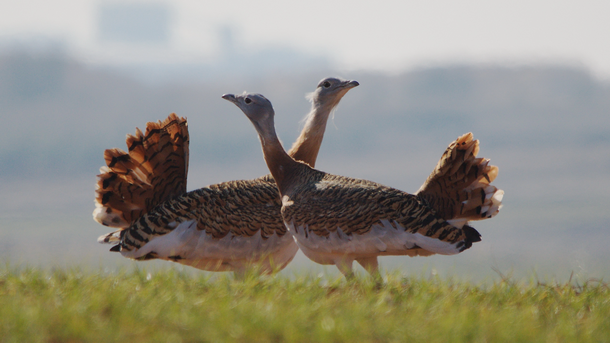
\includegraphics[width=10cm]{../fig/Cap12-Avutardas.png}
\end{enColor}
\begin{bn}
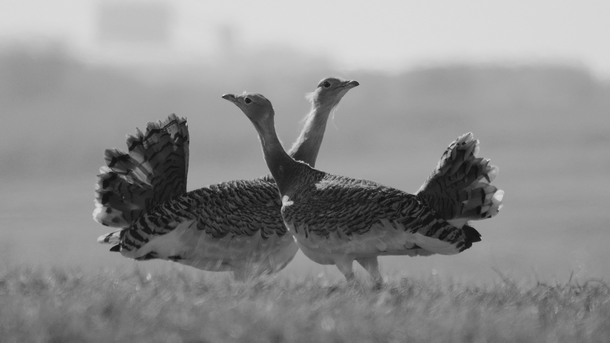
\includegraphics[width=10cm]{../fig/Cap12-Avutardas-bn.png}
\end{bn}
  \caption{Dos avutardas en la zona de Campo Real, Madrid.}
  \label{cap12:Fig:FotoAvutardas}
\end{center}
\end{figure}


\begin{Ejemplo}\label{cap12:ejem:Avutardas}
El campus externo de la Universidad de Alcalá linda con la ZEPA (zona de especial protección para
las aves) llamada {\em Estepas Cerealistas de los Ríos Jarama y Henares}. Ver el enlace [\,\ref{enlace0027}\,]\label{enlace0027a}, del
Ayuntamiento de Daganzo.



Este espacio protegido, junto con otras zonas similares de Madrid, alberga una importante población
de {\em Avutarda Común}\index{avutardas} ({\em Otis
tarda}, ver el enlace [\,\ref{enlace0028}\,]\label{enlace0028a}, de la Wikipedia), de la que forman parte los dos machos confrontados de la Figura
\ref{cap12:Fig:FotoAvutardas} (España acoge aproximadamente la mitad de la población mundial de
estas aves). En 1998 el grupo ornitológico SEO-Montícola
(ver el enlace [\,\ref{enlace0029}\,]\label{enlace0029a}) publicó, en el {\em Anuario Ornitológico
de Madrid}, un estudio (ver la referencia \cite{AvutardasMadrid} en la Bibliografía) sobre las
poblaciones de Avutardas  en varias zonas de la Comunidad de Madrid. La Tabla
\ref{cap13:Tabla:AvutardasValoresObservados} recoge algunos datos sobre la composición de las
poblaciones en cada zona (son datos parciales, adaptados para este ejemplo).
    \begin{table}[ht]
    \centering
    \begin{tabular}{rrrrr}
      \hline
     & MachosAdultos & Hembras & MachosJovenes & Suma \\
      \hline
      Talamanca & 53 & 177 & 14 & 244 \\
      Ribatejada & 16 & 68 & 7 & 91 \\
      Meco & 10 & 30 & 0 & 40 \\
      Daganzo & 18 & 108 & 12 & 138 \\
      Camarma - Daganzo & 34 & 79 & 12 & 125 \\
      Camarma & 17 & 41 & 5 & 63 \\
      Cobeña & 4 & 27 & 12 & 43 \\
      Campo Real & 38 & 74 & 12 & 124 \\
      Pinto & 28 & 57 & 6 & 91 \\
      Torrejón & 37 & 95 & 8 & 140 \\
      Estremera & 17 & 24 & 3 & 44 \\
      \hline
      Suma & 272 & 780 & 91 & 1143 \\
       \hline
    \end{tabular}
    \caption{Tabla inicial de valores observados por grupos para la población de avutardas.}\label{cap13:Tabla:AvutardasValoresObservados}
    \end{table}

Una pregunta que podemos hacernos a partir de estos datos es si la composición (es decir, la proporción de machos adultos, hembras y machos jóvenes) de las poblaciones en las distintas zonas es la misma. Es decir, si la composición de las poblaciones de avutardas es {\em independiente} de la zona en la que se sitúa esa población. Convertimos esto en la hipótesis nula de nuestro análisis:
    \[H_0=\left\{\mbox{
    \begin{minipage}{7.5cm} La composición, por grupos, de la población, es\\ independiente de la zona donde se sitúa.
    \end{minipage}
    }\right\}\]
Y vamos a someter a escrutinio esta hipótesis, frente a los datos observados, utilizando para ello un contraste $\chi^2$ de independencia. Empezamos, como siempre, explorando los datos. En la tabla podemos observar que, para algunas de las zonas, hay grupos que no alcanzan el límite inferior de cinco observaciones que hemos establecido para que el contraste $\chi^2$ sea válido. ¿Qué hacemos? No hemos tenido, hasta ahora, ocasión de hablar mínimamente de diseño experimental. Así que lo que sigue son sólo unas indicaciones, para poder seguir adelante con el ejemplo, y no deben entenderse como un análisis riguroso de esos datos ({!`}y que nos perdonen tanto los ornitólogos que nos lean, como las propias avutardas!). Una posibilidad, en estos casos, es agrupar varios niveles del factor hasta obtener un número suficiente de observaciones. Naturalmente, esto debe hacerse con algún criterio, que permita hacer algo más que ``salvar nuestras cuentas''. Se trata, ante todo, de que los niveles agrupados sigan teniendo sentido, en el contexto del problema que estamos estudiando. En este ejemplo, en particular, y dado que algunas de las zonas estudiadas son colindantes, podemos tratar de agruparlas, como si simplemente estuviéramos considerando zonas más amplias. Por supuesto, puede que esto no tenga sentido, por ejemplo, si no tenemos más información sobre los posibles desplazamientos de las avutardas entre unas zonas y otras. De hecho, en el estudio original se señala que con posterioridad se descubrió que los individuos de una de esas zonas (Loeches), eran en realidad individuos en tránsito hacia otras zonas, y que en otro caso (Estremera) se trataba probablemente de individuos de poblaciones situadas en otras provincias. En particular, hechas todas las salvedades anteriores, y para continuar con el ejemplo, nosotros vamos a eliminar esas dos filas de nuestra tabla, y a agrupar algunas de las otras zonas atendiendo a su situación en el mapa. La tabla reagrupada\footnote{Agrupamos a Meco con Camarma, y a Cobeña con Camarma-Daganzo} que vamos a usar es la tabla \ref{cap13:Tabla:AvutardasValoresObservados2}.

\begin{table}[ht]
\centering
\begin{tabular}{lcccc}
      \hline
     Zona & MachosAdultos & Hembras & MachosJovenes & Suma \\
      \hline
        1. Talamanca & 53 & 177 & 14 & 244 \\
        2. Ribatejada & 16 & 68 & 7 & 91 \\
        3. Daganzo & 18 & 108 & 12 & 138 \\
        4. Camarma-Daganzo-Cobeña & 38 & 106 & 24 & 168 \\
        5. Camarma-Meco & 27 & 71 & 5 & 103 \\
        6. Campo Real & 38 & 74 & 12 & 124 \\
        7. Pinto & 28 & 57 & 6 & 91 \\
        8. Torrejón & 37 & 95 & 8 & 140 \\
       \hline
      Suma & 255 & 756 & 88 & 1099 \\
       \hline
\end{tabular}
\caption{Tabla ({\sf agrupada}) de valores observados por grupos para la población de avutardas.}\label{cap13:Tabla:AvutardasValoresObservados2}
\end{table}
Y, como se ve, ya no hay ninguna entrada en la tabla menor que cinco. Esta es la tabla que vamos a
usar como tabla de valores observados; es decir, estos son, para este ejemplo, los valores $o_{ij}$
(y sus marginales asociados, los $o_{i\,+}$ y los $o_{+\,j}$).

Siguiendo con la exploración, una posible representación gráfica de este conjunto de datos es en
forma de gráfico de columnas apiladas\index{gráfico de columnas apiladas}\index{columnas apiladas, gráfico de}, como el de la parte (a) de la Figura \ref{cap11:Fig:ColumnasMosaicoAvutardas} (pág. \pageref{cap11:Fig:ColumnasMosaicoAvutardas}).

Hay una columna por cada zona, dividida en tres trozos que corresponden a los tres subgrupos. La altura de cada porción de la columna indica el porcentaje correspondiente a cada subgrupo.
\begin{figure}[p]
\begin{center}
\begin{enColor}
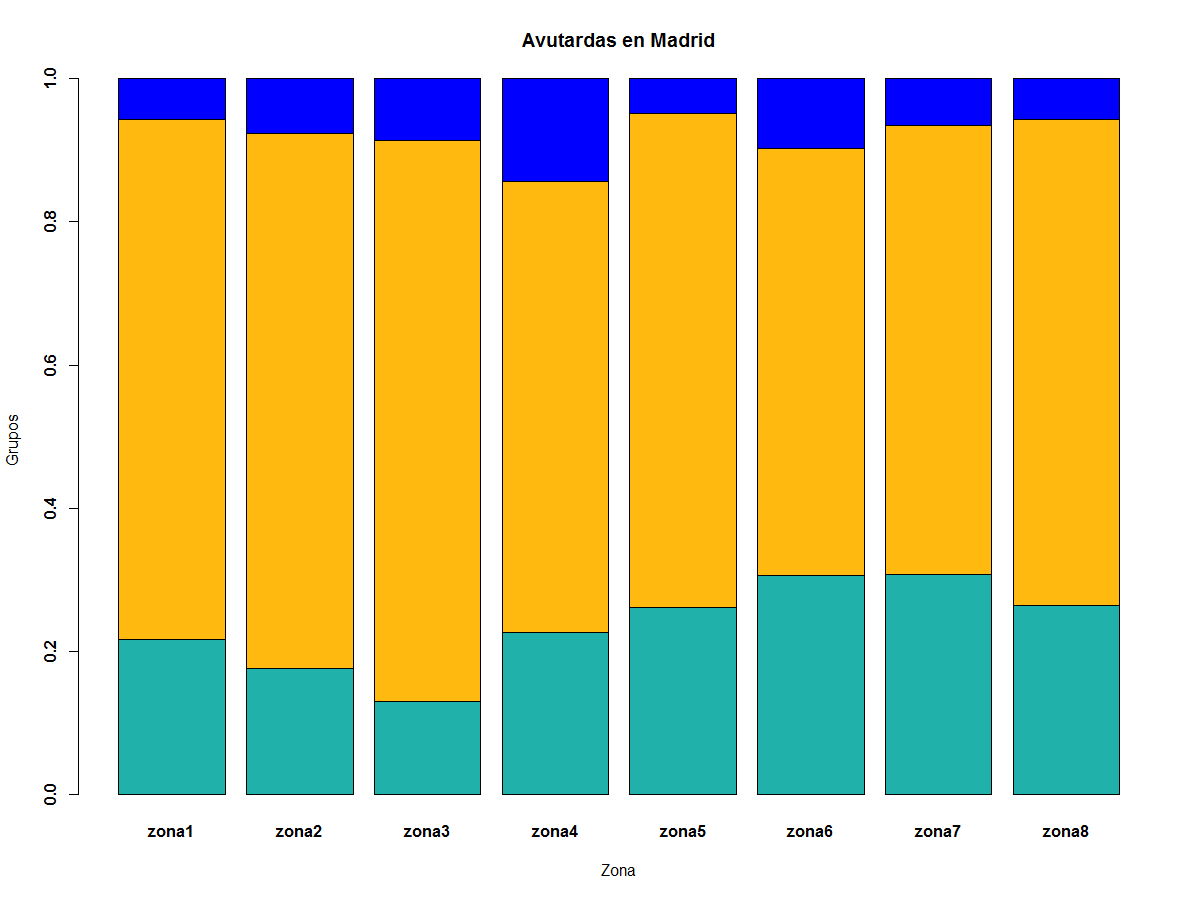
\includegraphics[width=12cm]{../fig/Cap12-Avutardas-Grafico01.png}\\
(a)\\
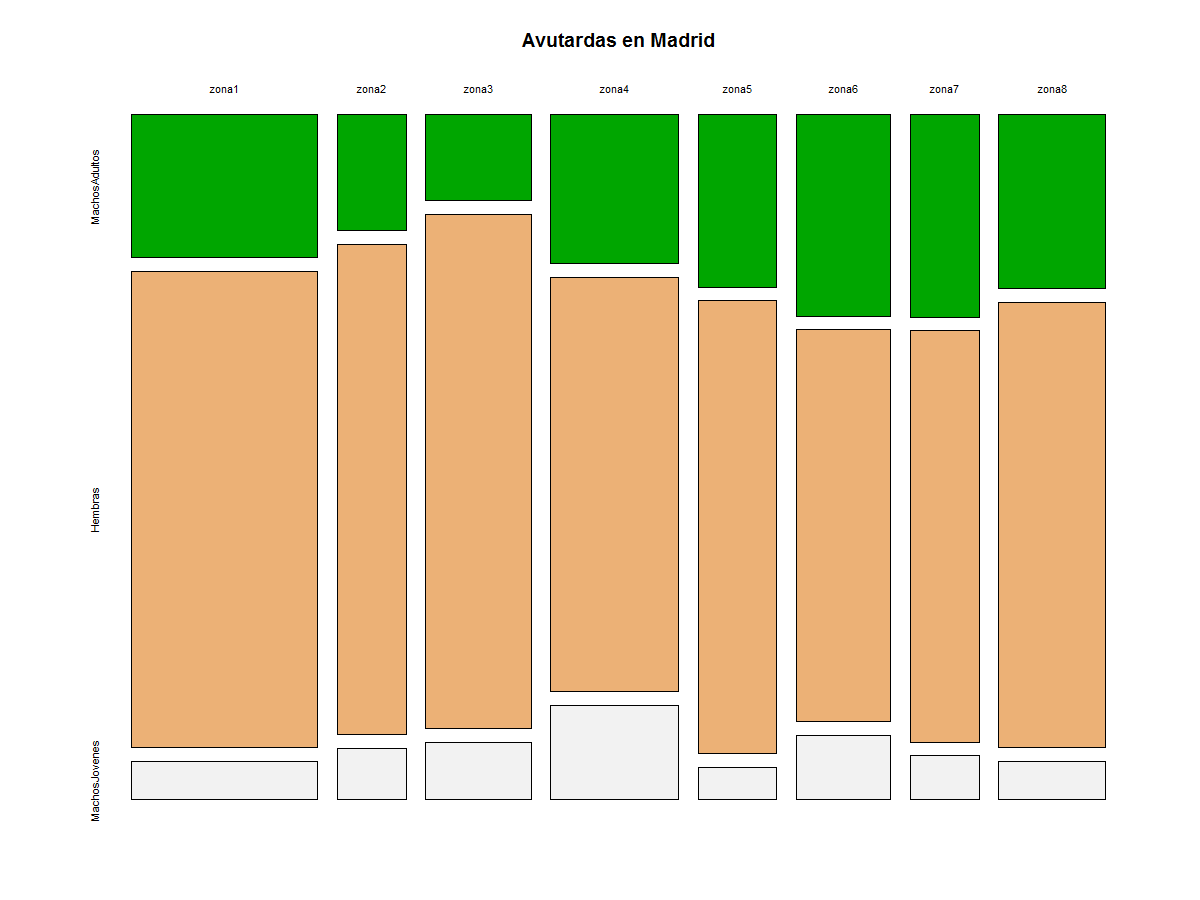
\includegraphics[width=12cm]{../fig/Cap12-Avutardas-Grafico02.png}\\
(b)\\
\end{enColor}
\begin{bn}
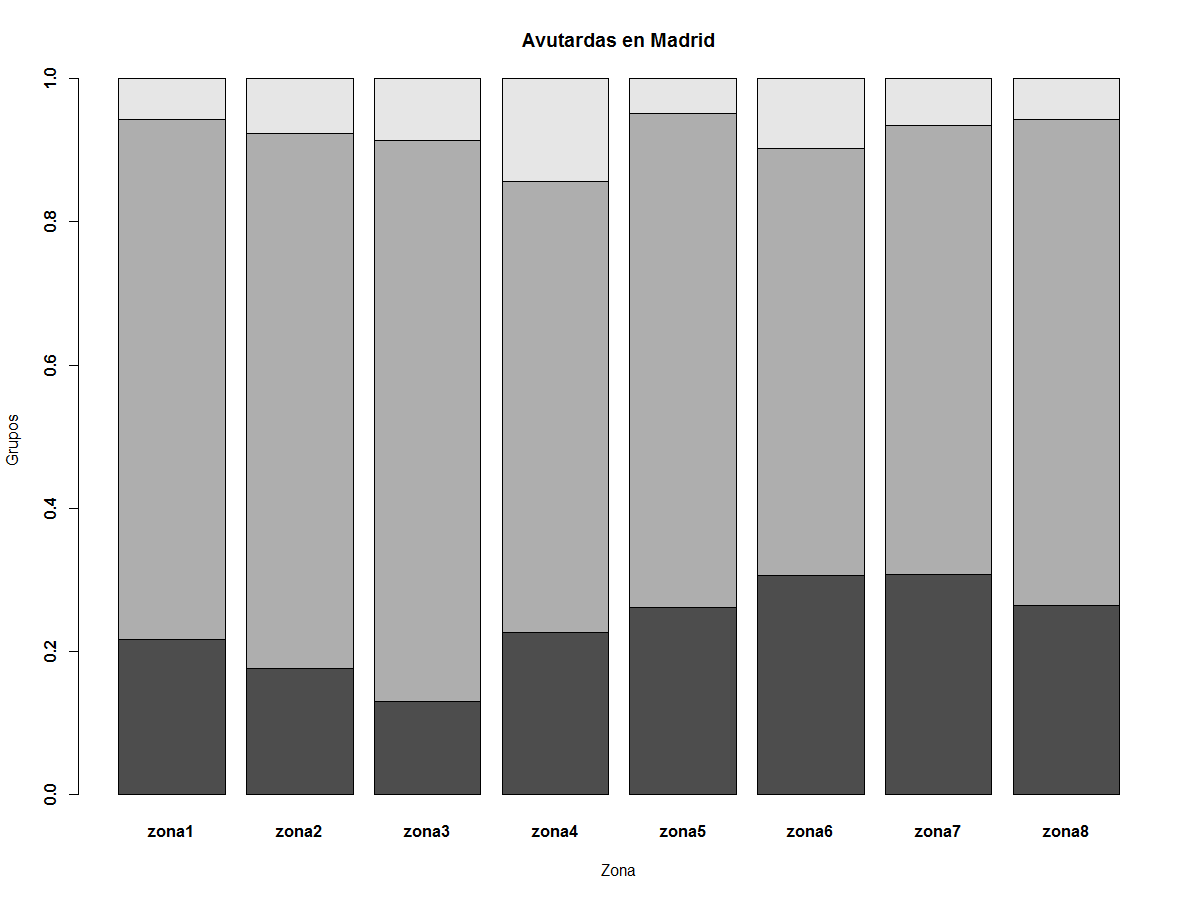
\includegraphics[width=12cm]{../fig/Cap12-Avutardas-Grafico01-bn.png}\\
(a)\\
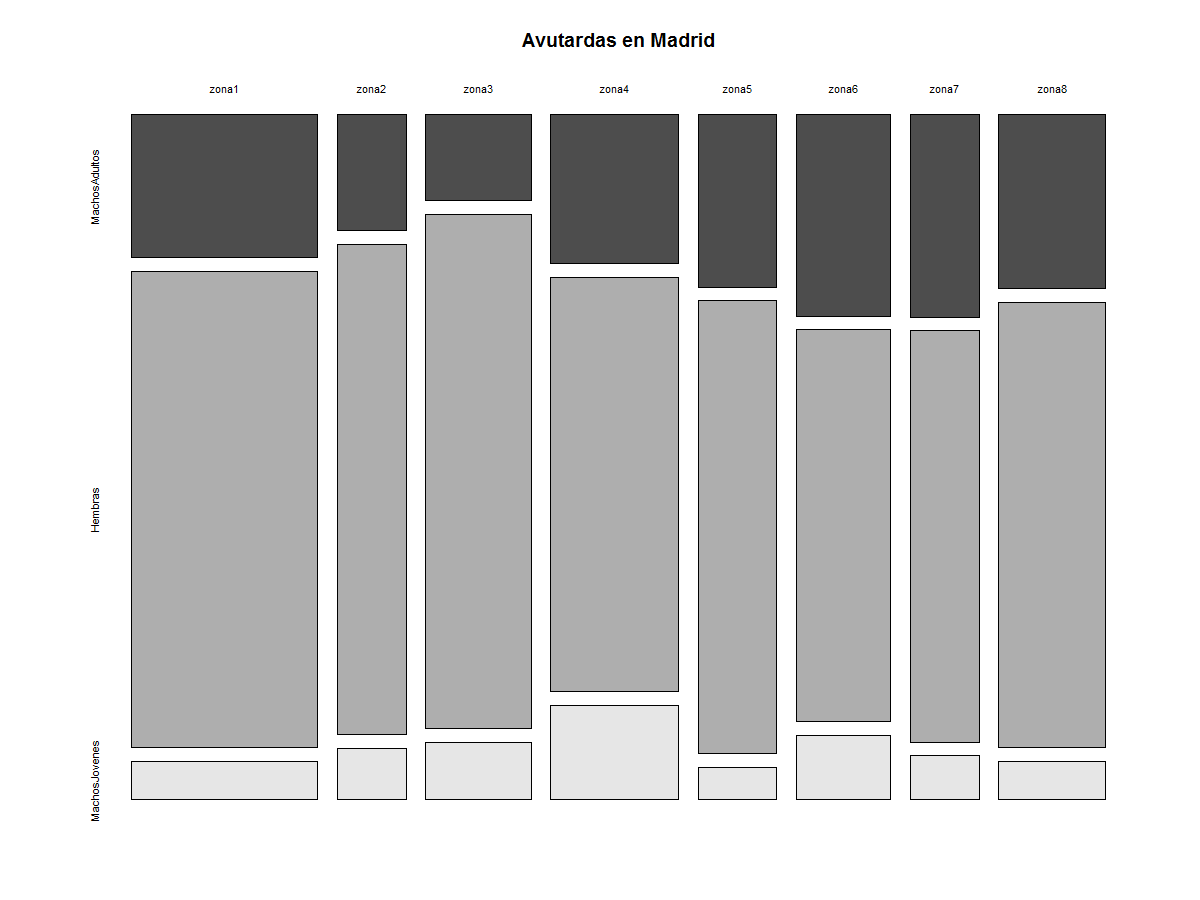
\includegraphics[width=12cm]{../fig/Cap12-Avutardas-Grafico02-bn.png}\\
(b)\\
\end{bn}
\caption{Gráficos de (a) columnas y (b) mosaico para el Ejemplo \ref{cap12:ejem:Avutardas}.}
\label{cap11:Fig:ColumnasMosaicoAvutardas}
\end{center}
\end{figure}
Otra variante, que aparece en la parte (b) de esa Figura, son los gráficos de mosaico\index{gráfico de mosaico}\index{mosaico, gráfico de} (en inglés, {\em mosaic plot}\index{mosaic plot}). En este tipo de gráficos, la anchura de las columnas es proporcional al tamaño de la correspondiente población de avutardas.


Como puede verse, la composición de las poblaciones es distinta, dependiendo de la zona que las
alberga. ¿Significativamente distinta? Para responder a esa pregunta vamos a seguir, paso a paso,
la construcción del contraste $\chi^2$. Partiendo de los valores marginales de esta tabla podemos
calcular una tabla de valores esperados $e_{ij}$, la Tabla
\ref{cap13:Tabla:AvutardasValoresEsperados} (pág. \pageref{cap13:Tabla:AvutardasValoresEsperados}).

    \begin{table}[h]
    \centering
    \begin{tabular}{lccc|r}
        \hline
        & MachosAdultos & Hembras & MachosJovenes & Suma \\
        \hline
        zona 1 & 56.62 & 167.85 & 19.54 & 244 \\
        zona 2 & 21.11 & 62.60 & 7.29 & 91 \\
        zona 3 & 32.02 & 94.93 & 11.05 & 138 \\
        zona 4 & 38.98 & 115.57 & 13.45 & 168 \\
        zona 5 & 23.90 & 70.85 & 8.25 & 103 \\
        zona 6 & 28.77 & 85.30 & 9.93 & 124 \\
        zona 7 & 21.11 & 62.60 & 7.29 & 91 \\
        zona 8 & 32.48 & 96.31 & 11.21 & 140 \\
        \hline
        Suma & 255 & 756 & 88 & 1099 \\
        \hline
    \end{tabular}
    \caption{Tabla de valores esperados por grupos para la población de avutardas.}\label{cap13:Tabla:AvutardasValoresEsperados}
    \end{table}
    Los valores de esta tabla se obtienen a partir de los marginales, como ya hemos visto en el comienzo de esta sección, de manera que:
    \[e_{ij}=\dfrac{o_{i\,+}\cdot o_{+\,j}}{n}.\]
    Por ejemplo,
    \[e_{32}=\dfrac{o_{3+}\cdot o_{+ 2}}{n}=\dfrac{138\cdot 756}{1099}\approx 94.93.\]

A partir de la Tabla \ref{cap13:Tabla:AvutardasValoresObservados2} y de la Tabla
\ref{cap13:Tabla:AvutardasValoresEsperados}, calculamos el estadístico:
    \[\Xi=\sum_{i=1}^{n_1}\sum_{j=1}^{n_2}\left(\dfrac{(o_{ij}-e_{ij})^2}{e_{ij}}\right).\]
donde $n_1=8$ es el número de zonas (filas de la tabla) y $n_j=3$ es el número de grupos
(columnas). En total tenemos que sumar 21 términos, y se obtiene:
    \[\Xi\approx 32.23084,\]
como valor del estadístico. Para obtener el p-valor del contraste debemos calcular la cola derecha
de la distribución $\chi^2$. ¿Con qué grados de libertad? A riesgo de ser pesados, vamos a intentar
de nuevo justificar la respuesta. Para ello, volvamos a la tabla, con los valores marginales, pero
supongamos que nos dan una colección {\em parcial} de valores observados, que ocupan las posiciones
que se representan con asteriscos en la Tabla \ref{cap13:Tabla:AvutardasGradosLibertad}.
\begin{table}[htb]
\centering
\begin{tabular}{lccc|c}
  \hline
 Zona & MachosAdultos & Hembras & MachosJovenes & Suma \\
  \hline
    zona 1 & * & * & ?? & 244 \\
    zona 2 & * & * & ?? & 91 \\
    zona 3 & * & * & ?? & 138 \\
    zona 4 & * & * & ?? & 168 \\
    zona 5 & * & * & ?? & 103 \\
    zona 6 & * & * & ?? & 124 \\
    zona 7 & * & * & ?? & 91 \\
    zona 8 & ?? & ?? & ?? & 140 \\
    \hline
    Suma & 255 & 756 & 88 & 1099 \\
   \hline
\end{tabular}
\caption{Ejemplo \ref{cap12:ejem:Avutardas}. Tabla para la determinación de los grados de libertad.}
\label{cap13:Tabla:AvutardasGradosLibertad}
\end{table}

Y supongamos que que sólo nos faltan los valores que corresponden a las interrogaciones. Está claro
que los valores que faltan (los símbolos ??) se pueden calcular a partir de los que ya tenemos (los símbolos *). Esto ilustra que, a la hora de rellenar una de estas tablas de contingencia, podemos elegir libremente
$(n_1-1)\cdot(n_2-1)$ valores, y esos son los grados de libertad que tenemos. En este ejemplo, eso
significa que debemos usar una distribución $\chi^2$ con $(8-1)\cdot(3-1)=14$ grados de libertad. Y
el p-valor que se obtiene, usando el ordenador, es aproximadamente $0.003714$. Como este p-valor
es bastante pequeño, podemos rechazar la hipótesis nula $H_0$, y afirmar que los datos apoyan la
hipótesis de que la composición de la población de avutardas depende de la zona en la que se
encuentra.
\qed
\end{Ejemplo}

Vamos a cerrar esta sección con algunos comentarios sobre el contraste $\chi^2$ de independencia, y sobre las tablas de contingencia que lo protagonizan.

\subsubsection*{Simetría del contraste $\chi^2$ de independencia.}

En los ejemplos que hemos visto, hemos dicho que íbamos a estudiar la posible relación de dependencia entre dos factores, en la forma $F_1 \sim F_2$. ¿Qué sucede si intercambiamos los papeles de $F_1$ y $F_2$? Absolutamente nada. Si el lector reflexiona sobre la forma de la Tabla \ref{cap12:tabla:tablaContingenciaGeneral} (pág. \pageref{cap12:tabla:tablaContingenciaGeneral}), se dará cuenta de que al cambiar $F_1$ y $F_2$ la tabla se traspone. Y otro tanto sucede con la tabla de valores esperados. Pero ni el valor del estadístico $\chi^2$ de la Ecuación \ref{cap12:ecu:EstadisticoChi2ParaTablasGenerales} (\pageref{cap12:ecu:EstadisticoChi2ParaTablasGenerales}), ni los grados de libertad que se usan en el contraste cambian al trasponer esas tablas. Así que el p-valor y la conclusión serán los mismos, sea cual el factor que se considere como {\em variable independiente}.

\subsubsection*{Tablas de contingencia relativas.}
\label{cap12:subsubsec:tablasContingenciaRelativas}

Las tablas de contingencia son similares, en el caso de dos factores, a las tablas de frecuencia que hemos usado desde el principio del curso, para los casos en que teníamos una única variable. Junto con las tablas de frecuencia, en la página \pageref{cap02:subsubsec:MedianaTablasFrecuenciasRelativasAcumuladas} del Capítulo \ref{cap:ValoresCentralesDispersion} introdujimos las tablas de frecuencias relativas, frecuencias acumuladas y frecuencias relativas acumuladas. En el caso de las tablas de contingencia no vamos a calcular valores acumulados. Sólo valores marginales, sumando por filas o columnas. Pero lo que sí tiene sentido es pensar en las frecuencias relativas, porque esas frecuencias relativas son, como hemos comentado en ocasiones, un objeto muy cercano a la idea de probabilidad.

La discusión que pretendemos plantear aquí no es nueva en el curso. Si el lector repasa el Ejemplo \ref{cap03:ejem:PruebasDiagnosticas01} (pág. \pageref{cap03:ejem:PruebasDiagnosticas01}), comprobará que en aquel caso ya estábamos calculando probabilidades a partir de una tabla de contingencia $2\times 2$. De hecho lo que calculábamos eran frecuencias relativas, pero cuando se tiene una muestra finita, y se eligen individuos de la muestra al azar, las probabilidades y las frecuencias relativas coinciden (gracias a la regla de Laplace).

En cualquier caso, queremos llamar la atención del lector sobre el hecho de que, dada una tabla de contingencia general, como la Tabla \ref{cap12:tabla:tablaContingenciaGeneral} (pág. \pageref{cap12:tabla:tablaContingenciaGeneral}), hay varias formas de {\em dividir por el total} en esa tabla, a diferencia de lo que sucede en una tabla de frecuencia simple.  Veámoslo en un ejemplo.
\begin{ejemplo}
\label{cap12:ejem:tablasContingenciaRelativas}	
Para no complicar las cosas, vamos a recuperar la tabla de contingencia $2\times 2$ del  Ejemplo \ref{cap03:ejem:PruebasDiagnosticas01} (pág. \pageref{cap03:ejem:PruebasDiagnosticas01}), que era:
    \begin{center}
    \begin{tabular}{|c|c|c|c|}
      \hline
      % after \\: \hline or \cline{col1-col2} \cline{col3-col4} ...
       &{\bf Enfermos }&{\bf Sanos }& Total \\
       \hline
      {\bf Positivo} & $192$&  $158$&  $350$\\
      \hline
      {\bf Negativo }&  $4$ & $9646$&  $9650$\\
      \hline
      Total    & $196$& $9804$& $10000$\\
      \hline
    \end{tabular}
    \end{center}
Para empezar, podemos dividir toda la tabla por el total $10000$. Se obtiene:
    \begin{center}
    \begin{tabular}{|c|c|c|c|}
      \hline
      % after \\: \hline or \cline{col1-col2} \cline{col3-col4} ...
       &{\bf Enfermos }&{\bf Sanos }& Total \\
       \hline
      {\bf Positivo} & $0.0192$ & $0.0158$ & $0.0350$ \\
      \hline
      {\bf Negativo }&  $0.0004$ & $0.9646$ & $0.9650$ \\
      \hline
      Total    & $0.0196$ & $0.9804$ & $1.000$ \\
      \hline
    \end{tabular}
    \end{center}
Las cuatro celdas de la tabla original (sin tener en cuenta los totales de los márgenes), suman $1$.  Por su parte, la columna de totales (a la derecha de la tabla), y la fila de totales (en la parte inferior), también suman $1$,  por separado en este caso. Algunos de estos valores ya se calcularon en el Ejemplo \ref{cap03:ejem:PruebasDiagnosticas01}, y allí se interpretaron como probabilidades, correctamente, en el sentido que hemos comentado.

Por otra parte, también podemos dividir cada fila de la tabla por la suma {\em de esa fila concreta}. Si hacemos eso, se obtiene esta tabla:
    \begin{center}
    \begin{tabular}{|c|c|c|c|}
      \hline
      % after \\: \hline or \cline{col1-col2} \cline{col3-col4} ...
       &{\bf Enfermos }&{\bf Sanos }& Total \\
       \hline
      {\bf Positivo} & $0.5486$ & $0.4514$ & $1$ \\
      \hline
      {\bf Negativo }&  $0.0004$ & $0.9996$ & $1$ \\
      \hline
    \end{tabular}
    \end{center}
Como puedes ver, hemos eliminado la fila inferior de totales. Lo hemos hecho porque, en el caso de esta tabla, las sumas por columnas no tienen ningún sentido. Cada fila se ha obtenido dividiendo por un denominador diferente ($350$ para la primera fila, $9650$ para la segunda). Y por lo tanto su suma no es interpretable en términos de probabilidades. Las sumas por columnas sí tienen sentido, pero ambas dan como resultado, obviamente, $1$. ¿Qué son, entonces, los valores que hemos obtenido al dividir así? Se trata, como el lector seguramente ha adivinado, de probabilidades condicionadas, en las que la condición es precisamente el suceso que corresponde a cada nivel del factor que aparece en las filas (en este ejemplo, el resultado de la prueba). Por ejemplo, en la celda intersección de la primera fila y primera columna, encontramos el valor
\[P\left(\mbox{enfermo} | \mbox{positivo}\right)=\dfrac{192}{350}\approx 0.5486,\]
que ya habíamos calculado en el Ejemplo \ref{cap03:ejem:PruebasDiagnosticas01}.

Desde luego, si dividimos cada columna de la tabla por la suma {\em de esa columna concreta}, obtendremos una tabla con las probabilidades condicionadas para cada uno de los niveles del factor que aparece en las columnas (que, en este ejemplo, es el factor que distingue entre enfermos y sanos). Dejamos como ejercicio para el lector calcular esa tabla, y compararla con algunas de las probabilidades condicionadas que calculamos en el Ejemplo \ref{cap03:ejem:PruebasDiagnosticas01}.
\qed
\end{ejemplo}
En el Tutorial12 aprenderemos a obtener estas {\sf tablas de contingencia relativas}\index{tablas de contingencia relativas}, o {\sf tablas de proporciones}\index{tablas de proporciones}, con ayuda del ordenador. Pero no queremos despedirnos de ellas sin poner en guardia al lector: a veces, en algunas publicaciones (sobre todo en las menos técnicas), se incluyen estas tablas sin especificar qué tipo de tabla se está mostrando. La forma infalible de detectar ante que clase de tabla estamos es sumando por filas o columnas. Si la suma de cada fila es $1$, estamos ante una tabla de probabilidades condicionadas para el factor correspondiente. Un comentario análogo sirve si la suma de cada columna es $1$. Y si es toda la tabla la que suma $1$, entonces estamos ante una tabla de probabilidades absolutas.

\section{El contraste de hipótesis $\chi^2$ de homogeneidad (para la bondad del ajuste).}
\label{cap12:sec:ChiCuadradoHomgeneidad}

\noindent En la segunda parte de este capítulo vamos a estudiar un problema íntimamente relacionado con lo que acabamos de aprender. De hecho, los dos problemas son tan similares en muchos aspectos que el principal riesgo que corre el lector es confundirlos. Vamos a tratar de subrayar claramente lo que
es igual y lo que es diferente. Empezaremos con un ejemplo muy sencillo (para algunas cosas, demasiado sencillo).

\begin{ejemplo}
\label{cap12:ejem:DadoCargado}
En el fichero adjunto
\fichero{../datos/Cap13-dado5000.csv}{Cap13-dado5000.csv} están
almacenados los resultados de 5000 lanzamientos de un dado. La Tabla \ref{cap12:tabla:valoresObservadosEjemploDadoCargado} muestra las de frecuencias, o valores observados,
correspondiente a esos 5000 lanzamientos.

\begin{table}[ht]
    \begin{center}
    \begin{tabular}{|l|c|c|c|c|c|c|}
      \hline
      % after \\: \hline or \cline{col1-col2} \cline{col3-col4} ...
      Resultado & 1 & 2 & 3 & 4 & 5 & 6 \\
      \hline
      Frecuencia & $o_1=811$ & $o_2=805$ & $o_3=869$ & $o_4=927$ & $o_5=772$ & $o_6=816$\\
      \hline
    \end{tabular}
    \end{center}
\caption{Tabla de frecuencias (valores observados) para el Ejemplo \ref{cap12:ejem:DadoCargado}}
\label{cap12:tabla:valoresObservadosEjemploDadoCargado}
\end{table}

¿No hay demasiados cuatros en esta tabla? ¿Significa eso que es un dado cargado? ¿Cómo podríamos averiguarlo?

¿En qué se parece este problema a la discusión de la sección previa? Bueno, para empezar tenemos una variable categórica, con seis factores que se corresponden con los seis posibles resultados al lanzar el dado. Y tenemos una tabla con frecuencias observadas, que podemos llamar
        \[o_1=811, o_2=805,\ldots, o_6=816.\]
Por supuesto, tenemos también en la cabeza un {\sf modelo teórico} de lo que esperamos que suceda con un dado no cargado, que corresponde con  nuestra asignación de probabilidad $1/6$ para cada uno de los posibles resultados. Es, de hecho, la idea misma de un dado no cargado en la versión {\em frecuentista} de la teoría de la Probabilidad. Es un dado que, al lanzarlo muchas veces, produce una tabla de frecuencias cada vez más parecida a la tabla ideal. ¿Y cuál es esa tabla ideal de frecuencias teóricas esperadas $e_i$, para los 5000 lanzamientos de un dado no cargado? El que aparece en la Tabla, \ref{cap12:tabla:valoresEsperadosEjemploDadoCargado} donde $\dfrac{5000}{6}\approx 833$.:

\begin{table}[htb]
{\small
        \begin{center}
        \begin{tabular}{|l|c|c|c|c|c|c|}
          \hline
          % after \\: \hline or \cline{col1-col2} \cline{col3-col4} ...
          Resultado & 1 & 2 & 3 & 4 & 5 & 6 \\
          \hline
          Frecuencia \rule{0cm}{0.6cm}& $e_1=\dfrac{5000}{6}$ & $e_2=\dfrac{5000}{6}$ & $e_3=\dfrac{5000}{6}$ & $e_4=\dfrac{5000}{6}$ & $e_5=\dfrac{5000}{6}$ & $e_6=\dfrac{5000}{6}$\\[2mm]
          \hline
        \end{tabular}
        \end{center}
}
\caption{Probabilidades esperadas para el Ejemplo \ref{cap12:ejem:DadoCargado}}
\label{cap12:tabla:valoresEsperadosEjemploDadoCargado}
\end{table}

Naturalmente, se trata de comparar la tabla esperada con la tabla observada, y ver si coinciden,
dentro de un margen que razonablemente podamos atribuir al azar. Porque, como hemos dicho, en la
tabla de frecuencias que abre esta sección parece que hay demasiados cuatros y pocos cincos. ¿Pero
son esas diferencias con el ideal suficientemente grandes para considerarlas {\sf significativas}?

Hasta aquí, las similitudes con el problema de la sección anterior deberían resultar obvias: hay
una tabla esperada, una tabla observada, y la hipótesis nula dirá que la tabla esperada describe
correctamente la distribución de probabilidad; es decir:
    \[H_0=\left\{\mbox{\small el dado no está cargado}\right\}=\left\{\mbox{\small la probabilidad de cada uno de los valores es $\dfrac{1}{6}$} \right\}\]
\qed
\end{ejemplo}

¿Cuál es entonces la diferencia entre el problema de este ejemplo y el de la sección previa? En la
sección previa estabamos estudiando {\em la posible relación entre dos variables categóricas (factores)} $F_1$
y $F_2$ (por ejemplo, género y creencias religiosas). Pero aquí sólo hay una variable, cuyo valor
es el resultado del lanzamiento del dado. Y lo que estamos tratando de decidir es {\em si los
valores observados se ajustan a una distribución teórica de probabilidades.} Esa es la diferencia
esencial entre las dos situaciones, que se traduce en una denominación distinta para lo que hacemos
en cada caso:
        \begin{itemize}
          \item El {\sf contraste (test) de independencia}\index{contraste de independencia, $\chi^2$}\index{$\chi^2$, contrastes de independencia y homogeneidad}\index{independencia, contraste $\chi^2$}\index{test $\chi^2$}\index{homogeneidad, contraste $\chi^2$}, que vimos en la sección anterior, usa la distribución $\chi^2$ para analizar la posible relación entre dos variables categóricas.
          \item El {\sf contraste (test) de homogeneidad}\index{contraste de homogeneidad, $\chi^2$}, que vamos a discutir en esta sección, es un contraste de hipótesis que usa la distribución $\chi^2$ (como veremos enseguida) para analizar si los valores observados se ajustan a una distribución teórica de probabilidades. Por esa razón, este contraste se llama también {\sf test de bondad del ajuste}\index{test $\chi^2$ de bondad del ajuste}\index{bondad del ajuste, $\chi^2$} (en inglés, {\em goodness of fit}\index{goodness of fit}).
        \end{itemize}


Como hemos dicho, vamos a aplicar la distribución $\chi^2$ para realizar un contraste de homogeneidad y
así poder decidir si el dado de nuestro ejemplo está o no cargado. Hay un primer paso muy fácil,
que el lector probablemente ya habrá anticipado. Puesto que se trata de un contraste de hipótesis,
tenemos que calcular un estadístico. Y en este caso, usaremos {\em ``el mismo''} que en el contraste de
independencia. Es decir, para cada celda de la tabla, calculamos el término:
    \[\dfrac{(\mbox{observado}-\mbox{esperado})^2}{\mbox{esperado}}\]
y sumamos todos esos términos.
\begin{ejemplo}
En concreto, para el ejemplo del dado, eso significa hacer esta
operación:

\[\Xi=\sum_{i=1}^6\frac{(o_i-e_i)^2}{e_i}=\dfrac{(o_1-e_1)^2}{e_1}+\cdots+\dfrac{(o_6-e_6)^2}{e_6}=\]

{\scriptsize
\[
\frac{(811-833)^2}{833}+\frac{(805-833)^2}{833}+\frac{(869-833)^2}{833}+\frac{(927-833)^2}{833}
+\frac{(772-833)^2}{833}+\frac{(816-833)^2}{833}\approx 18.49
\]
}
\qed
\end{ejemplo}

Seguramente el lector está pensando ``esto se ha acabado; ahora sólo tengo que usar la distribución
$\chi^2$ para calcular el p-valor''. Y, en efecto, así es {!`}salvo por un pequeño detalle! ¿Cuántos
grados de libertad vamos a usar en $\chi^2$?

Para responder a esa pregunta, lo mejor que podemos hacer es pensar de forma parecida a la que ya
vimos en el caso de la Tabla \ref{cap13:Tabla:AvutardasGradosLibertad} (página
\pageref{cap13:Tabla:AvutardasGradosLibertad}). Allí utilizamos los valores marginales para
establecer el número de grados de libertad. Concretamente, nos preguntábamos, una vez fijados esos
valores marginales, cuántos valores podíamos elegir de una forma arbitraria.
\begin{ejemplo}
¿Cuál es la situación
en el ejemplo de los 5000 lanzamientos del dado? Bueno, aquí sólo hay una fila en la tabla, y por
tanto, un único valor marginal, como hemos ilustrado en la Tabla \ref{cap12:tabla:GradosLibertadEjemploDadoCargado}.

\begin{table}[h!]
        \begin{center}
        \begin{tabular}{|l|c|c|c|c|c|c|c|}
          \hline
          % after \\: \hline or \cline{col1-col2} \cline{col3-col4} ...
          Resultado & 1 & 2 & 3 & 4 & 5 & 6 & Total\\
          \hline
          Frecuencia & ? & ? & ? & ? & ? & ? & 5000\\
          \hline
        \end{tabular}
        \end{center}
\caption{Grados de libertad para el Ejemplo \ref{cap12:ejem:DadoCargado}}
\label{cap12:tabla:GradosLibertadEjemploDadoCargado}
\end{table}

Hemos representado con interrogaciones las celdas donde debemos colocar los valores observados. Y queremos invitar al lector a que, antes de seguir leyendo, se detenga un momento en esa tabla y piense ¿cuántos de esos valores podemos escoger libremente? Otra manera de entender la pregunta (y acercarse a la respuesta) es esta: ¿qué condición o condiciones tienen que verificar esos números?

Desde luego, tienen que ser números enteros no negativos, y ninguno de ellos puede ser mayor que 5000. Pero hay muchísimas maneras de elegir seis números que cumplan esas condiciones. ¿De cuántas formas te puedes repartir 5000 euros con otros cinco amigos? Vamos a ver, pensemos un momento: 300 para A, 1000 para B, 500 para C,\ldots ¿Ya te has dado cuenta? No tropezamos con una barrera real hasta que hemos elegido cinco de los seis números. Pero en ese momento, al llegar al último número, descubrimos que ya no nos queda ningún margen de maniobra. Los grados de libertad son cinco.

Con esto hemos añadido el último ingrediente que necesitábamos para completar el contraste de
homogeneidad, y ya podemos calcular el correspondiente p-valor. Se trata de calcular la cola
derecha (¿por qué la derecha?) en la distribución $\chi^2_5$, para el valor del estadístico
$\Xi\approx 18.49$. Utilizando el ordenador se obtiene un p-valor que es aproximadamente
$0.0024$. Con este p-valor tan bajo podemos rechazar con bastante confianza la hipótesis nula, y
sospechar (fuertemente) que el dado está cargado.
%Como autor del programa con el que se han generado esos 5000 lanzamientos simulados, no me queda más remedio que confesar que, en efecto, había cargado el dado. Veremos en el Tutorial12 ese programa, y los cálculos de este ejemplo.
\qed
\end{ejemplo}


\subsubsection{Un ejemplo con probabilidades teóricas distintas entre sí}

El ejemplo del dado que hemos visto tiene, si acaso, la virtud de la sencillez. Pero esa misma
sencillez puede oscurecer un detalle importante. Por eso antes de seguir adelante, vamos a
presentar otro ejemplo, esta vez con menos detalle en los aspectos que no cambian con respecto al
caso del dado.
\begin{ejemplo}
\label{cap12:ejem:Mendel}
    En 1865, Gregor Mendel sentó las bases de la Genética como ciencia, en un artículo titulado {\em Versuche über Pflanzenhybriden} ({\em Experimentos sobre hibridación de plantas}, en el enlace [\,\ref{enlace0030}\,]\label{enlace0030a} puedes ver una versión completa, en inglés). Como aprende cualquier estudiante en un curso de Introducción a la Genética, G. Mendel\index{Mendel} estableció una serie de leyes de la herencia que permiten predecir características heredadas por una generación, a partir de la información sobre los genes de sus progenitores. Las leyes de Mendel predicen la {\em proporción} de descendientes que heredarán una cierta característica. No hacen, sin embargo (y hablando en general) predicciones individuales, y es esa razón la que hace que la Genética tenga, desde sus orígenes (grabado en sus genes, si se nos permite la broma) un vínculo especial con la Probabilidad y
    la  Estadística.
%    Remitimos al lector, por ejemplo, al libro {\em Las Matemáticas de la Vida} \link{http://www.planetadelibros.com/las-matematicas-de-la-vida-libro-60801.html}{http://www.planetadelibros.com/las-matematicas-de-la-vida-libro-60801.html}
%    \pendiente{(Añadir a la bibliografía)}
Pero concretando, y para no convertir este ejemplo en un curso de Genética, Mendel hizo muchos
experimentos con la planta del guisante (sobre todo, {\em Pisum Sativum}). Estas plantas presentan
semillas de dos formas distintas (lisas y rugosas). Usando sus leyes, y siguiendo un ingenioso y
meticuloso procedimiento experimental, Mendel, era capaz, con la ayuda de sus leyes, de predecir la
proporción de descendientes con semillas lisas o rugosas, en las sucesivas generaciones, a partir
de unos progenitores cuya dotación genética (genotipo) le era conocida. En uno de los experimentos
que se describen en ese artículo, Mendel vaticina usando sus leyes que, en los descendientes que
forman una determinada generación, la proporción
    \[\dfrac{\mbox{semillas lisas}}{\mbox{semillas rugosas}}\]
debía ser de 3 a 1. Esas son las {\em predicciones teóricas}, que vamos a comparar con lo que
sucedió cuando Mendel, de hecho, cultivó esas plantas. En concreto, Mendel obtuvo 7324 semillas
para esa generación. La proporción 3:1 esperada significa, traduciéndola en términos de
probabilidades
%\pendiente{relacionar esto con los dichosos odds}
que, de cada cuatro semillas, tres deberían ser lisas y la cuarta rugosa. Las probabilidades son:
    \[p_{lisa}=\dfrac{3}{4},\qquad p_{rugosa}=\dfrac{1}{4}.\]
Y precisamente el hecho de que estas probabilidades son distintas es el detalle por el que nos
hemos embarcado en este ejemplo. Recordemos que en el caso del dado cargado todas las probabilidades
teóricas eran iguales a $1/6$. Pero salvo por eso, el razonamiento es el mismo.  Como en los
ejemplos previos de este capítulo, obtenemos fácilmente una tabla de valores esperados:
    \begin{center}
    \begin{tabular}{|l|c|c|c|}
      \hline
      % after \\: \hline or \cline{col1-col2} \cline{col3-col4} ...
      Forma de la semilla & lisa & rugosa & total\\
      \hline
      Frecuencia \rule{0cm}{0.6cm}& $e_1=7324\cdot\dfrac{3}{4}=5493$ & $e_2=7324\cdot\dfrac{1}{4}=1831$ & 7324\\[2mm]
      \hline
    \end{tabular}
    \end{center}
Frente a esos valores esperados, Mendel obtuvo los valores observados que aparecen en esta tabla:
    \begin{center}
    \begin{tabular}{|l|c|c|c|}
      \hline
      % after \\: \hline or \cline{col1-col2} \cline{col3-col4} ...
      Forma de la semilla & lisa & rugosa & total\\
      \hline
      Frecuencia \rule{0cm}{0.6cm}& $o_1=5474$ & $o_2=1850$ & 7324\\[2mm]
      \hline
    \end{tabular}
    \end{center}
El resto es sencillo. Calculamos el estadístico:
    \[\Xi=\dfrac{(o_1-e_1)^2}{e_1}+\dfrac{(o_2-e_2)^2}{e_2}= \dfrac{(5474-5493)^2}{5493}+\dfrac{(1850-1831)^2}{1831}\approx 0.2629\]
y entonces usamos $\chi^2_1$ (con un grado de libertad; ¿por qué?; asegúrate de entender por qué es así) para calcular la probabilidad de la cola derecha definida por este valor (de nuevo, asegúrate
de entender porque es la cola derecha). Esto es, el p-valor del contraste. Se obtiene un p-valor
aproximado de $0.61$. A plena conciencia, y contra lo que sensatamente debe hacerse siempre, hemos
calculado el p-valor sin formular la hipótesis nula. Queremos que ese sea también un ejercicio para
el lector. ¿Cuál es la hipótesis nula que estábamos contrastando (nosotros, y Mendel, mirando con
sus gafillas redondas por encima de nuestro hombro)? Desde luego, con un p-valor tan grande, no vamos a rechazar esa
hipótesis. ¿Y por qué es eso una buena noticia para las teorías de Mendel?\flushright$\qed$
\end{ejemplo}

Ya estamos listos para enunciar más formalmente el contraste de homogeneidad:\\[3mm]

\fcolorbox{black}{Gris025}{
\begin{minipage}{12.5cm}
\begin{center}
    {\bf Contraste de hipótesis (test) $\chi^2$ de homogeneidad (Bondad del ajuste)}\\
    {\bf Caso de una variable discreta con un número finito de valores.}
\end{center}
    Sea $X$ una variable aleatoria discreta, que toma los valores $x_1,\ldots,x_k$ con probabilidades
    $p_1,\ldots,p_k$. Supongamos dada una muestra de tamaño $n$, con una tabla de valores (o frecuencias)
    observados:
        \begin{center}
        \begin{tabular}{|l|c|c|c|c|c|}
          \hline
          % after \\: \hline or \cline{col1-col2} \cline{col3-col4} ...
          Valor & $x_1$ & $x_2$ & $\cdots$ & $x_k$ &  Total \\
          \hline
          Frecuencia \rule{0cm}{0.6cm}& $o_1$ & $o_2$ & $\cdots$ & $o_k$ & $n$\\[2mm]
          \hline
        \end{tabular}
        \end{center}
    Y supongamos que queremos contrastar la hipótesis nula de que la muestra corresponde a la
    distribución definida por la variable $X$. Los {\em valores esperados} son:
        \[e_1= n\cdot p_1, e_2= n\cdot p_2,\ldots,e_k= n\cdot p_k.\]
        \begin{equation}
        \label{cap12:ecu:ContrasteChi2Homogeneidad}
        \mbox{Definimos el estadístico:\quad } \Xi=\dfrac{(o_{1}-e_{1})^2}{e_{1}}+\dfrac{(o_{2}-e_{2})^2}{e_{2}}+\cdots+\dfrac{(o_{k}-e_{k})^2}{e_{k}}.
        \end{equation}
    Entonces, {\sf mientras $n>30$ y ninguno de los valores $e_{i}$ sea menor de $5$}, el estadístico
    $\Xi$ sigue una distribución $\chi^2_{n-1}$, con {\sf n-1} grados de libertad.
\end{minipage}
}\\[3mm]

Como hemos indicado, este contraste $\chi^2$ de homogeneidad se denomina a menudo {\em contraste (o test) $\chi^2$ para la bondad del ajuste\index{bondad del ajuste, test $\chi^2$}} (en inglés, {\em goodness of fit}\index{goodness of fit}).

\section{El contraste exacto  de Fisher. Distribución hipergeométrica.}
\label{cap12:sec:ContrasteFisher}
\noindent{\bf Opcional: esta sección puede omitirse en una primera lectura.}\\

Como hemos señalado, el contraste $\chi^2$ de independencia, que hemos visto en la Sección \ref{cap12:sec:TablasContingencia}, está muy relacionado con el contraste de igualdad entre dos proporciones que vimos en la Sección \ref{cap09:sec:DiferenciaProporciones2Poblaciones} (pág. \pageref{cap09:sec:DiferenciaProporciones2Poblaciones}), cuya hipótesis nula es
\[H_0=\{p_1=p_2\}.\]
En esta sección llamaremos $p$ al valor común de las proporciones.

Por otra parte, ambos métodos, el del contraste $\chi^2$ y el de la Sección \ref{cap09:sec:DiferenciaProporciones2Poblaciones}, se basan, en última instancia, en la aproximación normal a las distribuciones binomiales que proporciona el Teorema Central del Límite. Y en ese fundamento común reside la debilidad de ambos métodos. En los dos casos ha sido necesario imponer condiciones sobre el tamaño de la muestra: ver las condiciones \ref{cap09:ecu:CondicionesInferenciaDiferenciaProporciones} (pág. \pageref{cap09:ecu:CondicionesInferenciaDiferenciaProporciones}) en el caso de la diferencia de proporciones, y las condiciones que acompañan al estadístico $\chi^2$ de la Ecuación \ref{cap12:ecu:EstadisticoChi2ParaTablasGenerales} (pág. \pageref{cap12:ecu:EstadisticoChi2ParaTablasGenerales}).

¿Pero qué ocurre cuando, a pesar de que $p$ tenga un valor moderado,  las muestras de las que disponemos son pequeñas? En ese caso, la aproximación normal no está justificada, y necesitamos un análogo del método exacto de Clopper y Pearson, que vimos en la Sección \ref{cap08:subsec:MetodoExactoBinomial} (pág. \pageref{cap08:subsec:MetodoExactoBinomial}). Ese método es el {\sf contraste exacto de Fisher}, que vamos a describir en esta sección. Como de costumbre, vamos a usar un ejemplo para guiar nuestros pasos. El contraste exacto de Fisher se utiliza a menudo en un contexto biosanitario (por ejemplo, en Epidemiología), como en el caso de las pruebas diagnósticas que hemos usado en varias ocasiones. Así que, por esa razón, y para que la intuición acompañe y ayude a la notación, vamos a usar la terminología de la {\sf exposición a un factor de riesgo}. Puedes pensar, por ejemplo, en que una parte de la población se ha expuesto a un contaminante presuntamente relacionado con el desarrollo de una enfermedad, mientras que otra parte no ha sido expuesta. Y nos preguntamos si, de hecho, la proporción de personas enfermas es distinta entre las que han sido expuestas y las que no. Por lo tanto, tendremos un factor llamado {\em Exposición}, con los niveles {\em expuesto} y {\em no expuesto}, y otro llamado {\em Enfermedad}, con los niveles {\em enfermo} y {\em sano}.
\begin{ejemplo}
\label{cap12:ejem:MetodoFisher01}
Se sospecha que el consumo de determinada sustancia psicotrópica, de reciente aparición, puede suponer un riesgo elevado de desarrollar cierta enfermedad. Se dispone de los datos que aparecen en la Tabla \ref{cap12:tabla:marginalesEjemploMetodoFisher02}. Como puede verse en la tabla, para evaluar la prueba se han usado dos muestras de personas, elegidas al azar, de las que $15$ consumen esa sustancia y $15$ no.
        \begin{table}[h!]
        \begin{center}
            \begin{tabular}{llccc}
            &&\multicolumn{3}{c}{\underline{\bf Exposición}}\\

                                      &          & Expuestos &  No Expuestos& Total\\
            \cline{2-5}
          \underline{\bf Enfermedad} & Enfermos & ??&  ??&   12\\
                                      & Sanos &  ?? & ??&  18\\
            \cline{2-5}
                                      & Total    & 15& 15& 30\\
            \cline{2-5}
            \end{tabular}
        \end{center}
        \caption{Tabla de contingencia para el Ejemplo \ref{cap12:ejem:MetodoFisher01}}
        \label{cap12:tabla:marginalesEjemploMetodoFisher01}
        \end{table}
Hemos omitido el contenido de las celdas centrales de la tabla, y sólo se muestran los valores marginales. A la vista de esos valores marginales, y con independencia del contenido de las otras celdas, parece claro que la dificultad es que no podemos usar el contraste $\chi^2$ en este ejemplo, porque el tamaño de la muestras es demasiado pequeño como para que el resultado sea fiable.
\qed
\end{ejemplo}

En ese ejemplo hemos dejado la Tabla \ref{cap12:tabla:marginalesEjemploMetodoFisher01} incompleta, al igual que hicimos con la Tabla \ref{cap12:tabla:marginalesEjemploBarometroCis} en el Ejemplo \ref{cap12:ejem:BarometroCIS01} (pág. \pageref{cap12:ejem:BarometroCIS01}), para insistir en que el problema es el mismo, y que lo que ha cambiado es el tamaño de las muestras. En general, nuestro punto de partida será una tabla $2\times 2$ de valores observados $o_{ij}$. De nuevo, como hicimos  entonces, queremos invitar al lector a que piense en las distintas formas de rellenarla. Es importante pensar en esto para entender la forma en la que vamos a plantear el contraste de hipótesis en este caso. ¿Cuál es la hipótesis que estamos contrastando?

Estamos suponiendo que hay dos poblaciones, expuestos y no expuestos. Y nos interesa, en ambas, la proporción de personas que enferman. Así que suponemos que las variables subyacentes a ambas poblaciones son de tipo Bernouilli, con proporciones $p_1$  (en expuestos) y $p_2$ (en no expuestos), respectivamente. Por lo tanto, si tomamos una muestra de una de esas poblaciones, el {\em número de enfermos en la muestra} será una binomial (como vimos en la discusión en torno a la Ecuación \ref{cap08:ecu:ProporcionMuestral}, pág. \pageref{cap08:ecu:ProporcionMuestral}). Los parámetros de la binomial son el tamaño de la muestra que tomemos, y la proporción en la población original, $p_1$ en el caso de los expuestos, o $p_2$ en el caso de los no expuestos.

Con ese lenguaje, la hipótesis alternativa que estamos contrastando se refiere a los valores $p_1$ y $p_2$:
\[H_a=\{p_1>p_2\}.\]
¿Cuál es el estadístico que vamos a usar? Para entenderlo, vamos a necesitar más maquinaria probabilística de la que hemos desarrollado hasta ahora en el curso. Y para ver porque eso es necesario, tenemos que volver a pensar en la Tabla \ref{cap12:tabla:marginalesEjemploMetodoFisher01}, y en su relación con la hipótesis nula
\[H_0=\{p_1\leq p_2\}.\]
Al fin y al cabo, la información muestral de la que dispondremos para realizar el contraste será una tabla como esta. ¿Cuál es el espacio muestral de {\em posibles tablas} en el que estamos pensando? No es una discusión trivial, y en su momento las decisiones que Fisher tomó al diseñar este contraste fueron objeto de bastante controversia entre los estadísticos. Puedes leer algo más sobre la discusión, y encontrar algunas referencias, en el enlace [\,\ref{enlace0031}\,]\label{enlace0031a} (en inglés).
Visto en perspectiva, la forma en la que Fisher planteó esto tal vez no sea la más {\em correcta}, desde el punto de vista formal, pero tiene la ventaja de la sencillez. Y en muchos casos, las respuestas que se obtienen por su método son comparables con las que proporcionan otros contrastes más elaborados. Remitimos al lector interesado en los detalles técnicos a los artículos de Cormack y Mantel (referencia \cite{cormack1991fisher}) y de Lydersen, Fagerland y Laake (referencia \cite{lydersen2009recommended}).

Para describir el contraste exacto de Fisher, vamos a utilizar una nueva notación para una tabla de contingencia $2\times 2$, que se ilustra en la Tabla \ref{cap12:tabla:notacionTablaContingenciaTestFisher}. Usamos esta notación, en lugar de la notación $o_{ij}$ y $e_{ij}$ de valores observados y esperados, porque, como se verá enseguida, en el contraste de Fisher vamos a emplear algunas tablas que no son ni observadas ni esperadas.  Por lo demás, la notación es muy parecida, y los subíndices $+$ indican valores marginales, obtenidos calculando la suma sobre una fila o columna, según la posición que ocupen.

\begin{table}[ht]
        \begin{center}
        \begin{tabular}{cc|c|c|c|}
              &\multicolumn{1}{c}{}&\multicolumn{3}{c}{\bf Exposición:}\\
              \cline{3-5}
              % after \\: \hline or \cline{col1-col2} \cline{col3-col4} ...
               &\multicolumn{1}{c|}{}& Expuestos&  No Expuestos& Total \\
               \cline{2-5}
        {\bf Enfermedad:}&\multicolumn{1}{|c|}{Enfermos}& $n_{11}$ & $n_{12}$ & $n_{1+}$ \\ % 11 8 19
              \cline{2-5}
             & \multicolumn{1}{|c|}{Sanos }& $n_{21}$ & $n_{22}$ &  $n_{2+}$\\ % 4  7 11
              \cline{2-5}
             & \multicolumn{1}{|c|}{Total} & $n_{+1}$ & $n_{+2}$ & $n$ \\
              \cline{2-5}
        \end{tabular}
        \end{center}
\caption{Notación para las tablas de contingencia que usamos en el contraste de Fisher}
\label{cap12:tabla:notacionTablaContingenciaTestFisher}
\end{table}

La decisión que tomó Fisher fue la de considerar {\em fijos los cuatro valores marginales:}
\[n_{1+},\quad n_{2+},\quad n_{+1},\quad n_{+2}.\]
Como hemos dicho, no es una decisión trivial. Esa condición de márgenes fijos no forma parte de la descripción inicial del problema, y puede plantear dificultades si, de hecho, tenemos una situación experimental en la que los márgenes no pueden considerarse fijos. Por lo tanto no vamos a tratar de convencer al lector de que es la mejor decisión posible (al fin y al cabo, hay buenos argumentos para justificar {\em otras posibilidades}). Pero sí vamos a tratar de hacer explícitas algunas de las ideas que se esconden detrás de esta decisión, para que el lector  sea consciente de lo que hacemos y dejamos de hacer. Después, cuando hayamos expuesto la forma de realizar el contraste de Fisher, haremos algunos comentarios adicionales sobre esto.

Para empezar, en muchas de las aplicaciones del contraste de Fisher, los tamaños de las dos muestras se consideran fijos (y a menudo, aunque no siempre, iguales), porque se ha establecido así {\em en el diseño del experimento}.  Eso explica porque Fisher pensaba en que los valores marginales,
      \[n_{+1},\quad n_{+2}\]
que en el contexto de las pruebas diagnósticas se refieren al tamaño de las muestras, son valores prefijados. Además, hemos dicho que nos estamos centrando en el caso de muestras pequeñas, y eso hace más fácil entender el interés en mantener fijo el tamaño de las muestras. Comparar una muestra de tamaño $10$ con  una de tamaño $15$ es más arriesgado (en términos de inferencia) que  comparar una de tamaño $1000$ con una de tamaño $1500$, aunque el incremento relativo sea el mismo en ambos casos. No obstante, en ocasiones, el diseño del experimento no considera fijo el tamaño de la muestra. Y en tales casos surge la duda de si el resultado del contraste de Fisher es un reflejo adecuado de la población. Para simplificar, como hemos dicho, vamos a suponer que estamos en uno de esos casos donde la hipótesis de tamaño muestral fijo es razonable.

Al fijar los tamaños muestrales, podemos terminar de concretar que las variables de interés en el contraste son las binomiales $X_1=B(n_{+1},p_1)$ y $X_2=(n_{+2},p_2)$, cuyo valor es, respectivamente, el número $n_{11}$ de enfermos en la muestra de la población $1$ (expuestos al factor de riesgo), o el número $n_{12}$ de enfermos en la población $2$ (no expuestos).


Supongamos, por lo tanto, que hemos fijado los tamaños de las muestras. Recuerda que estamos contrastando la hipótesis nula:
      \[H_0=\{p_1\leq p_2\}.\]
Como siempre, a la hora de hacer el contraste, suponemos que la hipótesis nula es cierta.  Pero, además, ya hemos dicho en varias ocasiones que, de entre todos los valores de los parámetros compatibles con la hipótesis nula, usaremos, para calcular los p-valores, aquellos que más favorezcan a $H_0$. Y, en este caso, está claro que eso implica suponer
      \[p_1=p_2.\]
Suponer esto significa que la exposición al factor de riesgo no cambia la proporción de personas enfermas. Y, si es así, las dos muestras de tamaños $n_{+1}$ y $n_{+2}$, que nosotros pensábamos que procedían de dos poblaciones distintas, en realidad forman, conjuntamente, una muestra de tamaño
\[n = n_{+1} + n_{+2}\]
de una población de tipo Bernouilli con proporción $p$, que es igual a ese valor común $p_1=p_2$. La suma marginal {\em de la primera fila} de la Tabla \ref{cap12:tabla:notacionTablaContingenciaTestFisher}:
\[n_{1+}=n_{11}+n_{12}\]
sirve, entonces, para construir un estimador muestral $\hat p$ de la proporción $p$:
\[\hat p=\dfrac{n_{1+}}{n}.\]
Así que una forma de justificar el razonamiento de Fisher es esta: una vez que $n$ está fijo (porque hemos fijado los márgenes inferiores de la tabla), al suponer que la hipótesis nula es cierta, el valor de $p$ (aunque sea desconocido) determina el valor de $n_{1+}$, y por lo tanto podemos suponer que $n_{1+}$ también es fijo. El último valor marginal restante $n_{2+}$ es, entonces, simplemente:
\[n_{2+}=n-n_{1+}.\]
En resumen, la justificación de los valores marginales fijos es que consideramos muestras de tamaño fijo, y que si la hipótesis nula de independencia es cierta, entonces $n_{1+}$ queda fijado por la proporción de casos expuestos en la población. En cualquier caso, si usamos el contraste exacto de Fisher, debemos tener en cuenta que estamos condicionando las probabilidades que calculamos a esos valores marginales fijos. Es decir, que el contraste exacto de Fisher que vamos a describir proporciona un p-valor {\em condicionado a los márgenes fijos} de la tabla de contingencia.

\begin{ejemplo}
\label{cap12:ejem:MetodoFisher02}
{\bf (Continuación del Ejemplo \ref{cap12:ejem:MetodoFisher01}).}
En la Tabla \ref{cap12:tabla:marginalesEjemploMetodoFisher01}, del Ejemplo \ref{cap12:ejem:MetodoFisher02}, el valor de $\hat p$ sería:
\[\hat p=\dfrac{12}{30}.\]
Si la aparición de la enfermedad es independiente del consumo de esa sustancia, esperaríamos que la proporción de enfermos fuera la misma en los expuestos y en los no expuestos. Es decir, que esperaríamos que fuera:
\[
n_{11}=15\cdot{\hat p}=15\cdot{\dfrac{12}{30}}=6,\qquad n_{12}=15\cdot{\hat p}=6.
\]
Así que, en caso de independencia, la tabla de contingencia esperada sería la Tabla \ref{cap12:tabla:marginalesEjemploMetodoFisher02}:
        \begin{table}[h!]
        \begin{center}
            \begin{tabular}{llccc}
            &&\multicolumn{3}{c}{\underline{\bf Exposición}}\\

                                      &          & Expuestos &  No Expuestos& Total\\
            \cline{2-5}
          \underline{\bf Enfermedad} & Enfermos & 6&  6&   12\\
                                      & Sanos &   9& 9&  18\\
            \cline{2-5}
                                      & Total    & 15& 15& 30\\
            \cline{2-5}
            \end{tabular}
        \end{center}
        \caption{Tabla de contingencia esperada en caso de independencia, para el Ejemplo \ref{cap12:ejem:MetodoFisher02}}
        \label{cap12:tabla:marginalesEjemploMetodoFisher02}
        \end{table}
\qed
\end{ejemplo}
Como puede verse, la situación nos recuerda a la del contraste $\chi^2$ de independencia.  Y en este punto estamos listos para ver la tabla muestral completa.
%Con esta notación, volvamos sobre la hipótesis que estamos contrastando. Si la hipótesis nula es cierta, la proporción de positivos en las dos poblaciones, sanos y enfermos, es la misma, a la que vamos a llamar simplemente $p$.  Supongamos que $o_{11}$, $o_{12}$ representan el número de positivos observados en las dos muestras. En ese caso, las proporciones muestrales:
%\[\hat p_1=\dfrac{o_{11}}{n_{+1}},\quad \hat p_2=\dfrac{o_{12}}{n_{+2}},\]
%son estimadores de $\hat p$.
\begin{ejemplo}
\label{cap12:ejem:MetodoFisher03}
{\bf (Continuación del Ejemplo \ref{cap12:ejem:MetodoFisher01}).}
La Tabla \ref{cap12:tabla:marginalesEjemploMetodoFisher03} contiene los valores muestrales que faltaban en la Tabla \ref{cap12:tabla:marginalesEjemploMetodoFisher01} (pág. \pageref{cap12:tabla:marginalesEjemploMetodoFisher03}).
        \begin{table}[h!]
        \begin{center}
            \begin{tabular}{llccc}
            &&\multicolumn{3}{c}{\underline{\bf Exposición}}\\

                                      &          & Expuestos &  No Expuestos& Total\\
            \cline{2-5}
          \underline{\bf Enfermedad} & Enfermos & 9&  3&   12\\
                                      & Sanos &   6& 12&  18\\
            \cline{2-5}
                                      & Total    & 15& 15& 30\\
            \cline{2-5}
            \end{tabular}
        \end{center}
        \caption{Tabla de contingencia para el Ejemplo \ref{cap12:ejem:MetodoFisher03}}
        \label{cap12:tabla:marginalesEjemploMetodoFisher03}
        \end{table}
Comparando esta tabla con la anterior Tabla \ref{cap12:tabla:marginalesEjemploMetodoFisher02}, se hace evidente que la proporción muestral de personas enfermas en la población expuesta es mayor que en la no expuesta. ¿Pero es significativamente mayor? ¿Cómo calculamos un p-valor?
\qed
\end{ejemplo}
La idea para el cálculo del p-valor es, en el fondo, la misma de siempre. Tenemos que suponer que la hipótesis nula es cierta, y usarla para calcular la probabilidad de obtener un resultado muestral como el que hemos obtenido, o más favorable aún a la hipótesis alternativa. Vamos a descomponer este problema en dos pasos.
\begin{itemize}
  \item En primer lugar, vamos a ver cuáles son esos posibles resultados muestrales más favorables a $H_a$.
  \item En segundo lugar (y esta es, con mucho, la parte que más trabajo nos va a dar) aprenderemos a calcular su probabilidad.
\end{itemize}

Veamos en un ejemplo como se da el primero de estos pasos.
\begin{ejemplo}
\label{cap12:ejem:MetodoFisher04}
{\bf (Continuación del Ejemplo \ref{cap12:ejem:MetodoFisher03}).}
Si pensamos en la Tabla \ref{cap12:tabla:marginalesEjemploMetodoFisher03}, entonces las tres tablas muestrales que aparecen agrupadas en la Tabla \ref{cap12:tabla:marginalesEjemploMetodoFisher04} son \underline{todas} las tablas muestrales posibles que son más favorables a $H_a$ que la Tabla \ref{cap12:tabla:marginalesEjemploMetodoFisher03}.

        \begin{table}[h!]
        \begin{center}
            \begin{tabular}{llccc}
            &&\multicolumn{3}{c}{\underline{\bf Exposición}}\\

                                      &          & Expuestos &  No Expuestos& Total\\
            \cline{2-5}
          \underline{\bf Enfermedad} & Enfermos & 10&  2&   12\\
                                      & Sanos &   5& 13&  18\\
            \cline{2-5}
                                      & Total    & 15& 15& 30\\
            \cline{2-5}
            \end{tabular}\\[3mm]


            \hrule
            \quad\\[3mm]

            \begin{tabular}{llccc}
            &&\multicolumn{3}{c}{\underline{\bf Exposición}}\\

                                      &          & Expuestos &  No Expuestos& Total\\
            \cline{2-5}
          \underline{\bf Enfermedad} & Enfermos & 11&  1&   12\\
                                      & Sanos &   4& 14&  18\\
            \cline{2-5}
                                      & Total    & 15& 15& 30\\
            \cline{2-5}
            \end{tabular}\\[3mm]

            \hrule
            \quad\\[3mm]

            \begin{tabular}{llccc}
            &&\multicolumn{3}{c}{\underline{\bf Exposición}}\\

                                      &          & Expuestos &  No Expuestos& Total\\
            \cline{2-5}
          \underline{\bf Enfermedad} & Enfermos & 12& \rule{0mm}{4mm} {\Large\bf 0}&   12\\
                                      & Sanos &   3& 15&  18\\
            \cline{2-5}
                                      & Total    & 15& 15& 30\\
            \cline{2-5}
            \end{tabular}

        \end{center}
        \caption{Tablas de contingencia más favorables a $H_a$ que la Tabla \ref{cap12:tabla:marginalesEjemploMetodoFisher03}, para el Ejemplo \ref{cap12:ejem:MetodoFisher04}}
        \label{cap12:tabla:marginalesEjemploMetodoFisher04}
        \end{table}

Fíjate en que los valores marginales son, en todas estas tablas, los mismos, como requiere la condición que impuso Fisher. ¿Por qué estamos seguros de que están son todas las tablas posibles? Pues por la forma en que las hemos construido.  Hemos partido de la Tabla \ref{cap12:tabla:marginalesEjemploMetodoFisher03} y en cada paso hemos aumentado en $1$ la posición $n_{11}$ de la tabla (la de la primera fila y primera columna). Y luego hemos calculado las tres posiciones restantes de la tabla, a partir de $n_{11}$ y de los valores marginales fijos. Naturalmente, al aumentar $n_{11}$, para que las sumas marginales se mantengan, los valores $n_{12}$ y $n_{12}$ tienen que disminuir. Pero no pueden ser negativos, así que al ir aumentando $n_{11}$ llega un momento en que uno de esos dos valores se hace cero. En nuestro caso el primero que alcanza el valor cero es $n_{12}$, como hemos destacado en la tercera de estas tablas. En ese momento podemos estar seguros de que tenemos la lista completa de tablas muestrales más favorables a $H_a$ que la tabla \ref{cap12:tabla:marginalesEjemploMetodoFisher03}.
\qed
\end{ejemplo}

El procedimiento descrito en este ejemplo nos permite construir la colección completa de tablas muestrales, con valores marginales fijos, que son tan favorables o más a $H_a$ que la tabla muestral de partida. El siguiente paso consiste en asignar una probabilidad a cada una de esas tablas. Puesto que cada una de esas tablas muestrales representa un suceso incompatible con cualquier tabla distinta, el p-valor será simplemente la suma de las probabilidades de esas tablas que hemos obtenido.

Pero ¿cómo vamos a calcular la probabilidad de obtener cada una de esas tablas? En este paso, como habíamos anunciado, necesitamos una herramienta nueva, una distribución de probabilidad discreta que no habíamos encontrado hasta ahora. Dedicaremos el próximo apartado a familiarizarnos con ella y, después, cuando veamos su relación con este problema, volveremos al punto donde nos hemos quedado, para completar el cálculo del p-valor.


\subsection{La distribución hipergeométrica.}
\label{cap12:subsec:DistribucionHipergeometrica}

Vamos a examinar un problema de Combinatoria muy relacionado con algunos de los que hemos visto en la Sección \ref{cap03:sec:Combinatoria} (pág. \pageref{cap03:sec:Combinatoria}) y con la construcción de la distribución binomial (ver Sección \ref{cap05:sec:ExperimentosBernouilliDistribucionBinomial}, pág. \pageref{cap05:sec:ExperimentosBernouilliDistribucionBinomial}).

Supongamos dada una caja con un total de $N$ bolas, de las cuales $B$ son blancas. Vamos a extraer una muestra de $m$ bolas de la caja, {\bf sin reemplazamiento}, y nos preguntamos por la probabilidad de que $k$ de las bolas extraídas sean blancas. Más concretamente, llamamos $X$ a la variable aleatoria
\[X=\mbox{\em (número de bolas blancas que hay entre las $m$ extraídas).}\]
Entonces nuestro problema es calcular esta probabilidad:
\[P(X=k).\]
Empezamos por hacer dos observaciones:
\begin{enumerate}
  \item Hemos usado $m$ y no $n$ para la muestra por razones que quedarán claras pronto, cuando volvamos al problema del contraste exacto de Fisher.
  \item El hecho de que el muestreo sea sin reemplazamiento es esencial. Si se considera muestreo con reemplazamiento, entonces obtendríamos una distribución binomial $B(n,p)$, siendo
    \[p=\dfrac{B}{N}\]
    la {\em proporción} de bolas blancas en la caja. Hacer el muestreo con reemplazamiento, como se hace en la binomial, implica, por tanto, que lo único importante será la proporción de bolas blancas, y que el número total de bolas en la caja $N$ será irrelevante. Cuando no hay reemplazamiento, en cambio, el valor de $N$ es determinante en el cálculo de probabilidades.
\end{enumerate}
Para resolver ese problema sólo necesitamos la regla de Laplace y algo de la Combinatoria que hemos aprendido. Empecemos por pensar en cuántos resultados elementales (equiprobables) hay, y luego veremos cuantos de ellos son favorables al suceso {\em ``la muestra extraída contiene $k$ bolas blancas''}. Para contar el número de sucesos elementales posibles debemos preguntarnos cuántas muestras de tamaño $n$ se pueden extraer sin reemplazamiento, de una caja con $N$ bolas, cuando no nos importa el orden en que se extraen esas bolas. El orden no importa porque las bolas blancas no se distinguen entre sí. Así que el orden en que se extraen no afecta a la equiprobabilidad (dejamos al lector que piense en los detalles, y en cómo hacer el cálculo teniendo en cuenta el orden de extracción; el resultado será el mismo, en cualquier caso). Teniendo esto en cuenta, la respuesta es:
\[\binom{N}{m}.\]
Ahora, para contar el número de sucesos favorables, tenemos que pensar cuántas formas hay de elegir las $k$ bolas blancas que componen la muestra, de entre las $B$ bolas blancas de la caja. De nuevo, no nos importa el orden, así que el número es:
\[\binom{B}{k}.\]
Pero con esto, sólo hemos elegido las bolas blancas que componen la muestra. {\em Para cada una de estas elecciones}, debemos elegir las $m-k$ bolas negras de la muestra, de entre las $N-B$ bolas negras de la caja. Eso se puede hacer de
\[\binom{N-B}{m-k}\]
maneras, así que reuniendo todo en la Regla de Laplace, vemos que la probabilidad que buscábamos es:
\[\dfrac{\dbinom{B}{k}\cdot\dbinom{N-B}{m-k}}{\dbinom{N}{m}}.\]
Vamos a llamar $X$ a la variable aleatoria cuyo valor es el número de bolas blancas que contiene la muestra. Es un nuevo tipo de variable aleatoria que no habíamos usado hasta ahora.
\begin{center}
    \fcolorbox{black}{Gris025}{
    \begin{minipage}{12cm}
        \begin{center}
        %%%%%%%%%%%%%%%%%%%%%%%%%%%%%%%%%%%%%%%
        {\bf  Variable aleatoria hipergeométrica.}
        \end{center}
        \index{variable aleatoria hipergeométrica}
        %%%%%%%%%%%%%%%%%%%%%%%%%%%%%%%%%%%%%%%
        La variable aleatoria discreta $X$ es {\sf hipergeométrica con parámetros $N$, $B$ y $m$} (todos enteros no negativos), lo que representaremos con el símbolo $Hyp(N,B,m)$, si su función de densidad viene dada por:
		\begin{equation}
        \label{cap05:ecu:DensidadHipergeometrica}
            \displaystyle P(X=k)=\dfrac{\dbinom{B}{k}\cdot\dbinom{N-B}{m-k}}{\dbinom{N}{m}}.
        \end{equation}
        Obsérvese que debe ser $B\leq N$, $m\leq N$ y $0\leq k\leq m$.
       \vspace{1mm}
        %%%%%%%%%%%%%%%%%%%%%%%%%%%%%%%%%%%%%%%
    \end{minipage}}
    \end{center}
En el Tutorial12 veremos como calcular esta función de densidad de la distribución hipergeométrica usando el ordenador.

La propia construcción de la distribución hipergeométrica hace evidente que las variables de este tipo aparecen cuando se estudia la distribución muestral de una proporción en una población, al tomar muestras sin reemplazamiento. Como hemos dicho, cuando las muestras se toman con reemplazamiento, este mismo problema conduce a la distribución binomial. Por esa razón vamos a ver con más detalle la relación que existe entre ambas variables.

\subsubsection{Relación entre hipergeométrica y binomial, y consecuencias muestrales.}

Supongamos que, con la notación que hemos introducido para discutir la distribución hipergeométrica, extraemos, como antes, $m$ bolas, pero ahora {\em con reemplazamiento}. La variable $\tilde X$ que describe el número de bolas blancas de la muestra es entonces una binomial $B(m,p)$, siendo
\[p=\dfrac{B}{N}\]
la proporción de bolas blancas en la caja. Llamamos como antes $X$ a la variable hipergeométrica, que corresponde al muestreo sin reemplazamiento. Queremos comparar $X$ con $\tilde X$, a medida que el
número $N$ total de bolas en la caja va aumentando, pero de manera que la proporción $p$ de bolas blancas
se mantiene constante (y no es excesivamente pequeña, en el mismo sentido que en la discusión de la distribución de Poisson). Si pensamos en el muestreo con reemplazamiento (variable binomial $\tilde X$), la intuición nos dice que, cuando $N$ se hace muy grande comparado con $m$, la probabilidad de seleccionar dos veces la misma bola, en una misma muestra, llegará a ser muy pequeña.  Por lo tanto, la inmensa mayor parte de las muestras con reemplazamiento son muestras cuyos elementos no se repiten, y que por tanto se podrían haber obtenido en un muestreo sin reemplazamiento. Es decir, que a medida que $N$ crece, manteniendo $p$ constante, las funciones de densidad de $X$ y $\tilde X$ se hacen cada vez más y más parecidas.
    \begin{center}
        \fcolorbox{black}{Gris025}{\begin{minipage}{12cm}
        \begin{center}
        {\bf Relación entre la distribución hipergeométrica y la binomial}
        \end{center}
            Si $N$ se hace muy grande, manteniendo la proporción $p=\dfrac{B}{N}$ constante (y con $p$ no demasiado pequeña), entonces
            \[Hyp(N,B,m)\sim B(m,p).\]
        \end{minipage}}
    \end{center}
En particular, este hallazgo tiene consecuencias prácticas a la hora de obtener muestras aleatorias de una población. Cuando se selecciona una muestra para un control de calidad, o un ensayo clínico, etc., a menudo no se cumple con esa condición ideal de muestra con reemplazamiento. Por falta de recursos, porque resulte inviable hacerlo o, simplemente, porque no se ha tenido en cuenta eso. En cualquier caso, sea cual sea el motivo por el que se ha obtenido una muestra sin reemplazamiento, debe tenerse en cuenta que si el tamaño $N$ de la población que muestreamos es muy grande comparado con el tamaño de la muestra, entonces la diferencia entre muestreo con y sin reemplazamiento es básicamente irrelevante para la validez de las conclusiones estadísticas, siempre que las muestras se obtengan de forma aleatoria.\\

Para los lectores matemáticamente más escrupulosos, es posible comprobar de una manera más formal esta relación entre la distribución hipergeométrica y la binomial. El razonamiento es mucho más técnico de lo que es habitual en este curso. Pero lo vamos a incluir aquí, porque no nos ha resultado posible encontrar una referencia a este argumento (que no fuera un enlace en Internet), y porque, aunque la idea que se persigue está clara, los pasos que hay que dar son algo intrincados. Si no te interesan especialmente estos detalles técnicos, te recomendamos encarecidamente pasar directamente al siguiente apartado. Si te quedas con nosotros, te esperan dos páginas de cuentas más o menos farragosas; estás advertido.

Empezamos escribiendo la función de densidad \ref{cap05:ecu:DensidadHipergeometrica} (pág. \pageref{cap05:ecu:DensidadHipergeometrica}) de la distribución hipergeométrica en términos de los factoriales:
\[
P(X=k)=\dfrac{\dbinom{B}{k}\cdot\dbinom{N-B}{m-k}}{\dbinom{N}{m}}=
\dfrac{
\dfrac{B!}{k!(B-k)!}\dfrac{(N-B)!}{(m-k)!(N-B-m+k)!}}{\dfrac{N!}{m!(N-m)!}}.
\]
Ahora reorganizamos esta expresión para hacer aparecer el número combinatorio $\binom{m}{k}$ que aparece en la binomial $B(m,p)$. Para ello hay que tomar el primer factor del denominador en cada uno de los tres números combinatorios. Luego, reorganizamos los términos:
\[
P(X=k)=\dfrac{m!}{k!(m-k)!}\cdot
\dfrac{
\frac{B!}{(B-k)!}\frac{(N-B)!}{(N-B-(m-k))!}}{\frac{N!}{(N-m)!}
}=
\dbinom{m}{k}\cdot
\frac{ B!}{N!(B-k)!}\cdot\frac{(N-B)!(N-m)!}{(N-B-(m-k))!}
.
\]
El siguiente es el paso ingenioso. Vamos a reorganizar esas dos fracciones de factoriales para que resulte evidente su relación con los términos
\[p^k\cdot q^{m-k}\]
de la binomial.  Hay que usar un par de trucos ingeniosos, pero la idea que hay detrás de lo que vamos a hacer es la misma que nos condujo a la Ecuación \ref{cap03:ecu:expresionPseudoFactorialCoeficientesBinomiales} (pág. \pageref{cap03:ecu:expresionPseudoFactorialCoeficientesBinomiales}). Una expresión de la forma:
\[\dfrac{R!}{(R-S)!},\]
donde $R$ y $S\leq R$ son numeros naturales, representa los primeros $S$ factores del factorial de $R$, y por lo tanto, se puede escribir en la forma:
\begin{equation}
\label{cap12:ecu:expresionPrimerosTerminosFactorial}
\dfrac{R!}{(R-S)!}=\underbrace{R\cdot(R-1)\cdot(R-2)\cdots(R-S+1)}_{S\mbox{ factores}}=
\prod_{i=1}^S (R-S+i)
\end{equation}
Y para poder aplicar esta relación a nuestro problema, multiplicamos y dividimos $P(X=k)$ por $(N-k)!$ (ese es el primer truco ingenioso).
\[
P(X=k)=
\dbinom{m}{k}\cdot
\frac{\dfrac{B!}{(B-k)!}}{\dfrac{N!}{(N-k)!}}\cdot\frac{\dfrac{(N-B)!}{(N-B-(m-k))!}}{\dfrac{(N-k)!}{(N-m)!}}
.
\]
Para poder aplicar cuatro veces la Ecuación \ref{cap12:ecu:expresionPrimerosTerminosFactorial}, vamos a sumar y restar $k$ en el denominador del último cociente de factoriales de esta expresión (ese es el segundo truco ingenioso):
\[
P(X=k)=
\dbinom{m}{k}\cdot
\frac{\dfrac{B!}{(B-k)!}}{\dfrac{N!}{(N-k)!}}\cdot\frac{\dfrac{(N-B)!}{(N-B-(m-k))!}}{\dfrac{(N-k)!}{(N-k-(m-k))!}}
.
\]
Y ahora sí, aplicando cuatro veces la Ecuación \ref{cap12:ecu:expresionPrimerosTerminosFactorial}, tenemos:
\[
P(X=k)=
\dbinom{m}{k}\cdot
\dfrac{\displaystyle\prod_{i=1}^k (B-k+i)}{\displaystyle\prod_{i=1}^k (N-k+i)}\cdot
\dfrac{\displaystyle\prod_{j=1}^{(m-k)} ((N-B)-(m-k)+j)}{\displaystyle\prod_{j=1}^{(m-k)}(N-m+j)}.
\]
Hemos usado $i$ com índice de los dos productos de la primera fracción, porque ambos recorren los valores de $1$ a $k$. Y hemos usado $j$ en los productos de la segunda fracción porque ambos recorren los valores de $1$ a $m-k$. Prácticamente hemos acabado. Basta con agrupar los productos de cada fracción aprovechando que comparten el recorrido de $i$ y $j$ respectivamente:
\begin{equation}
\label{cap12:ecu:DemostracionHipergeometricaBinomial01}
P(X=k)=
\dbinom{m}{k}\cdot
\displaystyle\prod_{i=1}^k\left(\dfrac{ B-k+i}{N-k+i}\right)
\cdot
\displaystyle\prod_{j=1}^{(m-k)}\left(\dfrac{(N-B)-(m-k)+j}{N-m+j}\right).
\end{equation}
Fíjate ahora en uno de los términos:
\[\dfrac{ B-k+i}{N-k+i}.\]
Puesto que $N$ es mucho más grande que $m$, y $k<m$, podemos estar seguros de que
\[\dfrac{ B-k+i}{N-k+i}\approx\dfrac{B}{N}=p.\]
Para convencerte, prueba a sustituir unos valores típicos, como podrían ser, por ejemplo,  $N=100000$, $B=30000$, $k=15$, $i=6$. Cuanto mayor sea la diferencia de tamaño entre $N$ y $m$, más evidente es esto. Y para el segundo producto, se tiene, de forma análoga:
\[\dfrac{(N-B)-(m-k)+j}{N-m+j}\approx\dfrac{N-B}{N}=\dfrac{N-N\cdot p}{N}=1-p=q.\]
Así que, sustituyendo esas aproximaciones en la Ecuación \ref{cap12:ecu:DemostracionHipergeometricaBinomial01}, se obtiene lo que queríamos:
\[
P(X=k)=\dbinom{m}{k}\cdot p^k\cdot q^{(m-k)}\approx P(\tilde X=k),
\]
siendo $\tilde X$ la binomial $B(n,p)$, que corresponde al muestro  con reemplazamiento.

En la práctica se suele admitir que la aproximación de la hipergeométrica por la binomial es válida cuando \[N > 10\cdot m.\]
Y no podemos cerrar  este apartado sin señalar que, como consecuencia del Teorema Central del límite, estos resultados implican que para $m$ grande ($m>30$), pero pequeño comparado con $N$, y para $p$ no demasiado pequeño, se tiene
\[Hyp(N,B,m)\sim B(m,p)\sim N(m\cdot p,\sqrt{m\cdot p\cdot q}).\]


\subsection{Aplicación de la distribución hipergeométrica al contraste exacto de Fisher.}
\label{cap12:subsec:RelacionHipergeometricaTablasContingencia}

Ahora que ya hemos visto la relación hipergeométrica, su relación con la binomial, y las consecuencias para la teoría muestral en poblaciones finitas estamos listos para: (a) confesar que esa es la principal razón que nos ha llevado a incluir el contraste exacto de Fisher en este capítulo (b) usar lo que hemos aprendido sobre esta distribución para volver al contraste exacto de Fisher en el punto donde lo dejamos, y terminar el cálculo del p-valor  de ese contraste.

La segunda razón para incluir el contraste de Fisher tiene que ver precisamente con la aplicación de la hipergeométrica. Tenemos la sensación de que, en muchas ocasiones, cuando se describe el método, esta parte se cubre con poco detalle, y que eso puede generar algunos mal entendidos y confusiones, que a la larga dificultan la aplicación correcta del método.

La dificultad, a nuestro juicio, es que en este problema hay que pensar en tres niveles, que vamos a tratar de describir.

Recordemos que, en el contraste exacto de Fisher, la hipótesis nula (de independencia) dice que en realidad no hay diferencia entre {\em expuestos} y no {\em expuestos}, en cuanto a la proporción de casos de enfermedad que aparecen en ambas poblaciones, que es la misma en ambos casos, y que vale $p$.
\begin{enumerate}
  \item Así que, por un lado está la población de la que tomamos muestras, y en la que hay esa proporción $p$ de enfermos. Desconocemos el tamaño de la población, y queremos dejar claro que el tamaño de la población {\em NO}\, es el número $N$ de la distribución hipergeométrica, sino un número en general mucho mayor.
  \item En esa población tomamos una muestra de tamaño $n$. En realidad, son dos muestras, una formada por $n_{+1}$ expuestos, y otra por $n_{+2}$ no expuestos, con
      \[n=n_{+1}+n_{+2}.\]
      Pero, para quien asuma que la hipótesis nula es cierta, no hay diferencia entre ambas. Esa muestra de tamaño $n$ va a jugar el papel de la caja de la distribución hipergeométrica. Así que, de hecho, lo que vamos a hacer es tomar $N=n$ en la hipergeométrica. Por eso, al presentar esa distribución hemos usado $m$ y no $n$, para tratar de evitar la confusión al llegar a este punto. Esa caja (la muestra de $n$ individuos en total) está compuesta por $n_{+1}$ individuos expuestos, que juegan el papel de las $B$ bolas blancas, y por $n_{+2}$ individuos no expuestos, que son las bolas negras de la caja.
      \begin{ejemplo}
      \label{cap12:ejem:MetodoFisher05}
      En el Ejemplo \ref{cap12:ejem:MetodoFisher04}, tendríamos $N=n=30$, mientras que
      \[B=n_{+1}=15,\qquad N-B=n_{+2}=15.\]
      \qed
      \end{ejemplo}
      Y aquí viene una observación importante: la hipótesis de Fisher de márgenes fijos implica, en el caso de los márgenes inferiores de la tabla, que la composición de la caja esta fijada, exactamente como se requiere para poder usar la distribución hipergeométrica.

  \item El tercer nivel es la {\em ``muestra''} de $m$ bolas que extraemos en la caja, en el modelo de la hipergeométrica, y que es esencial no confundir con la muestra de la población que hemos extraído en el paso anterior. La ``muestra'' de $m$ bolas, en el contraste de Fisher, corresponde a los $n_{1+}$ enfermos que componen nuestra muestra (esta, sin comillas, es la muestra de verdad, la de $n$ personas). Recordemos que Fisher nos dice que consideremos ese número como un número fijo. Y eso es lo que, a su vez, nos permite aplicar la distribución hipergeométrica a este problema, porque el número de bolas que extraemos de la caja es un número fijo. El valor $k$, que en la hipergeométrica es el número de bolas blancas que han salido de la caja, se traduce en el modelo de Fisher en el número de personas expuestas que han enfermado, el elemento $n_{11}$ de la tabla de contingencia.
      \begin{ejemplo}
      \label{cap12:ejem:MetodoFisher05}
      En el Ejemplo \ref{cap12:ejem:MetodoFisher04}, tenemos
      \[m=12,\]
      mientras que, en la tabla muestral \ref{cap12:tabla:marginalesEjemploMetodoFisher03} (pág. \pageref{cap12:tabla:marginalesEjemploMetodoFisher03}). Es decir, que estamos usando un modelo de una distribución hipergeométrica $X\sim Hyp(N,B,m)$ con
      \[N=30,\quad B=15,\quad m=12, \]
      y, para saber cuál es la probabilidad de una tabla muestral como la Tabla \ref{cap12:tabla:marginalesEjemploMetodoFisher03}, en la que $k=9$, nos preguntamos por la probabilidad
      \[
        P(X=9)=\dfrac{\dbinom{B}{k}\cdot\dbinom{N-B}{m-k}}{\dbinom{N}{m}}=
          \dfrac{\dbinom{15}{9}\cdot\dbinom{30-15}{12-9}}{\dbinom{30}{12}}\approx  0.02633
      .\]
      \qed
      \end{ejemplo}

\end{enumerate}
Confiamos en que las explicaciones anteriores hayan contribuido a aclarar un poco la forma en la que la distribución hipergeométrica se aplica a la situación del contraste exacto de Fisher. A riesgo de ser pesados, insistimos en que el mayor riesgo de confusión procede del hecho de dos nociones distintas de {\em muestra}, que intervienen en este caso. Una muestra de la población que estamos estudiando se convierte en una ``caja'' de la distribución hipergeométrica. El hecho de fijar los márgenes en la tabla de contingencia se traduce en que: (a) Estamos considerando muestras (o ``cajas'') siempre con la misma composición de individuos expuestos y no expuestos (bolas blancas y negras).  (b)  El número de bolas que se sacan de la caja (el número de individuos expuestos enfermos, y que es el otro concepto de ``muestra'' que interviene) es siempre el mismo para todas las muestras.

Vistas así las cosas, está claro que el contraste de Fisher selecciona, de entre todas las muestras de tamaño $n$ que podríamos extraer de la población, un subconjunto bastante particular. No sólo el número de individuos expuestos está fijo, sino también el número de enfermos. Ya hemos explicado antes las razones por las que Fisher creía que esta clase concreta de muestras era el espacio muestral adecuado para contrastar la hipótesis nula de independencia.

Para tratar de ayudar al lector a seguir esta discusión, en la Tabla \ref{cap12:tabla:TraduccionFisherHipergeometrica} hemos incluido una especie de {\em diccionario} de notación, para facilitar el paso de la distribución hipergeométrica a la tabla de contingencia del contraste exacto de Fisher y viceversa.

\begin{table}[ht]
        \begin{center}
        \begin{tabular}{|c|c|c|c|}
          \cline{2-4}
          % after \\: \hline or \cline{col1-col2} \cline{col3-col4} ...
           \multicolumn{1}{c|}{}& Bolas blancas&  Bolas negras & Total \\
           \hline
          Salen de la caja& $k$ & $m-k$ & $m$ \\
          \hline
          Quedan en la caja& $B-k$ & $(N-B)-(m-k)$ &  $N-m$\\
          \hline
          \multicolumn{1}{|c|}{Total} & $B$ & $N-B$ & $N$ \\
          \hline
        \end{tabular}\\[3mm]

        \hrule
        \quad\\[3mm]

        \begin{tabular}{|c|c|c|c|}
          \cline{2-4}
          % after \\: \hline or \cline{col1-col2} \cline{col3-col4} ...
           \multicolumn{1}{c|}{}& Expuestos&  No expuestos & Total \\
           \hline
          Enfermos& $n_{11}$ & $n_{12}$ & $n_{1+}$ \\
          \hline
          Sanos& $n_{21}$ & $n_{22}$ &  $n_{2+}$\\
          \hline
          \multicolumn{1}{|c|}{Total} & $n_{+1}$ & $n_{+2}$ & $n$ \\
          \hline
        \end{tabular}

        \end{center}
\caption{Tabla de ``traducción'' entre la notación de la tabla de contingencia del contraste exacto de Fisher, y la que hemos usado para el modelo de la distribución hipergeométrica}
\label{cap12:tabla:TraduccionFisherHipergeometrica}
\end{table}

%Otro de los aspectos que al principio pueden resultar confusos en relación con el contraste exacto de Fisher es el hecho de que este método no parece prestar ninguna atención a la proporción de personas expuestas en la población. Al fijar el tamaño de los márgenes inferiores, $n_{+1}$ y $n_{+2}$, de la tabla, hemos {\em impuesto}, como parte del diseño experimental, el reparto del número de casos de cada clase que se examinan en la muestra. Esto puede resultar chocante, pero, una vez más, debemos recordar que, al contrastar la hipótesis nula de independencia, lo hacemos  suponiendo que esa hipótesis es cierta. Y, si es cierta, entonces, los expuestos y no expuestos son iguales, en lo que refiere a la proporción de casos de enfermedad. Eso implica, en particular, que los tamaños muestrales que consideramos deberían ser irrelevantes.

\subsubsection{Cálculo del p-valor en el contraste exacto de Fisher}

Una vez entendida la conexión con la distribución hipergeométrica, el cálculo del p-valor se reduce a aplicar esa distribución para calcular la probabilidad de todas las tablas de contingencia que corresponden a un resultado muestral como el que hemos obtenido, o más favorable aún a la hipótesis alternativa. Veamos esto en el Ejemplo que hemos venido usando en esta sección.

\begin{ejemplo}
\label{cap12:ejem:MetodoFisher06}
{\bf (Continuación del Ejemplo \ref{cap12:ejem:MetodoFisher03}).}

En la Tabla \ref{cap12:tabla:marginalesEjemploMetodoFisher03} (pág. \pageref{cap12:tabla:marginalesEjemploMetodoFisher03}), del Ejemplo \ref{cap12:ejem:MetodoFisher03}, el número de individuos expuestos enfermos era igual a $9$. Posteriormente, en la Tabla \ref{cap12:tabla:marginalesEjemploMetodoFisher04} hemos mostrado otras tres tablas de contingencia que
corresponden a valores más favorables a la hipótesis alternativa, y hemos argumentado que esas son todas las tablas posibles. Así pues, teniendo en cuenta esto, y usando cálculos con la distribución hipergeométrica $X\sim Hyp(30, 15, 12)$, como en el Ejemplo \ref{cap12:ejem:MetodoFisher05}, se obtiene un p-valor igual a:
\[\mbox{p-valor}=P(X=9)+P(X=10)+P(X=11)+P(X=12)\approx
\]
\[
0.02632+0.003645+0.0002367+0.000005261\approx 0.03022
\]
Así que, si trabajamos con un nivel de significación del $95\%$, este p-valor nos permite rechazar la hipótesis nula de independencia, y concluir que la proporción de enfermos es distinta entre individuos expuestos y no expuestos.
\qed
\end{ejemplo}
En el Tutorial12 aprenderemos a ejecutar el test de Fisher con el ordenador de una forma sencilla.
